\documentclass[12pt]{article}
\usepackage[utf8]{inputenc}
\usepackage[brazil]{babel}
\usepackage{setspace}
\usepackage[T1]{fontenc}
\usepackage{a4,times,color}
\usepackage{textcomp}
\usepackage{amsmath}
\usepackage{amsfonts}
\usepackage{amsthm}
\usepackage{physics}
\usepackage{stackrel}
\usepackage{wasysym}
\usepackage{cancel}
\usepackage{pst-all}
\usepackage{caption}
\usepackage{floatrow}
\usepackage{xcolor}
\usepackage{color}
\usepackage{enumitem}
\floatsetup[table]{capposition=top}
\usepackage{bm}
\usepackage{empheq}



\oddsidemargin -1,5cm
\topmargin -3.cm
\textheight 27cm
\textwidth 19.cm
\onehalfspacing


\newcommand{\beq}{\begin{equation}}
\newcommand{\eeq}{\end{equation}}
\newcommand{\bse}{\begin{subequations}}
\newcommand{\ese}{\end{subequations}}
\newcommand{\bea}{\begin{eqnarray}}
\newcommand{\eea}{\end{eqnarray}}
%
\def\ie{{\it i.e.} }
%



\usepackage{natbib}
\usepackage{graphicx}

\begin{document}

{\centerline {\large {\colorbox{lightgray}{{\textcolor {blue} {\bf Experimento 3}}} }}

\vskip 0.3cm 

\large{ {\colorbox{lightgray}{{\textcolor {blue} {\bf Movimento de um corpo em queda vertical: determinação da aceleração da queda }}} \\
\hskip 0.5cm \large{ {\colorbox{lightgray}{{\textcolor {blue} {\bf e comparação com a aceleração da gravidade.}}} }}}}}

% -----------------------------------------------------------------------------------------------------------------------------
%\section{}
% -----------------------------------------------------------------------------------------------------------------------------
\indent

Neste experimento determinaremos a aceleração de um corpo em queda vertical e vamos 
comparar o resultado obtido com o valor de referência da aceleração da gravidade ($g$)
para a cidade de Rio de Janeiro. 
\par
Vamos analisar o movimento de queda vertical de um corpo cuja forma e tamanho apresente uma força de resistência do ar desprezível (por exemplo uma bolinha de gude)\footnote{Lembre que a queda vertical de um corpo quando a única força atuante sobre ele é a força da gravidade chama-se queda livre.}. Que tipo de movimento 
apresentaria o corpo se a força de resistência do ar fosse desprezível?\footnote{Lembre que o movimento da partícula é determinado através da Segunda Lei de Newton.}
\par 
Pense sobre o planejamento desse experimento. A aceleração do corpo pode ser obtida diretamente? Quais grandezas devem ser medidas para que seja possível obtê-la? Quais instrumentos são mais adequados para que esses dados possam ser coletados?
\par 
O experimento será discutido e guiado pelo roteiro abaixo. Siga o roteiro e as orientações do professor 
nos encontros remotos e vá fazendo suas anotações no caderno de laboratório. 

% ----------------------------------------------------------------------------
\section{Procedimento Experimental}
% ----------------------------------------------------------------------------

\begin{minipage}[c]{11.5cm}

\hskip 0.5cm
O arranjo experimental experimental está mostrado ao lado. Escolha uma bola de gude ou qualquer corpo arredondado de dimensões da ordem de grandeza da bolinha mostrada na figura ao lado. Você deverá filmar a queda da bolinha com um celular, desde uma altura de, mais o menos, um metro. Para isso peça ajuda a uma pessoa que vai segurar a bolinha enquanto você filma.  Cole na parede uma régua de papel como está indicado na figura \footnote{A régua não precisa ter a extensão de toda a trajetória a ser filmada. É somente uma referencia de escala.}. Para a filmagem posicione o celular num apoio com a tela do celular paralela à parede onde está colada a régua de papel. O celular deverá estar posicionado mais o menos no meio da trajetória da bolinha a uma distância da parede suficiente para poder filmar toda a queda de mais ou menos um metro. Não use ``slow-motion'' (câmera lenta),  filme com a velocidade normal do seu celular. A imensa maioria dos celulares filma a uma taxa de 30 frames/seg \footnote{A palavra em inglês ``frame'' significa quadro.}. Verifique no seu celular se essa é a taxa usada.
\par
\hskip 0.5cm
Para analisar o filme da queda será usado o aplicativo Tracker para uso num computador 
que poderá ser baixado gratuitamente no endereço eletrônico {\color{blue} https://physlets.org/tracker/
}\footnote{O aplicativo é disponibilizado para os sistemas operacionais Windows, Linux e Mac OSX.}. Alternativamente o filme poderá ser analisado com o aplicativo VidAnalysis disponível gratuitamente para celulares com sistema operacional Android no link  {\color{blue} https://play.google.com/store/apps/details?id=com.vidanalysis.free}. 
Os tutoriais de uso destes aplicativos estão disponíveis na forma de vídeos no site da disciplina dentro do site do Instituto de Física da UFRJ. No Apêndice \ref{ApendiceB} também poderá consultar um tutorial básico do aplicativo Tracker e no Apêndice \ref{ApendiceC}  poderá consultar um tutorial básico do aplicativo VidAnalysis.
\end{minipage}
\hskip 0.2cm
\begin{minipage}[c]{7cm}
\hskip 1cm
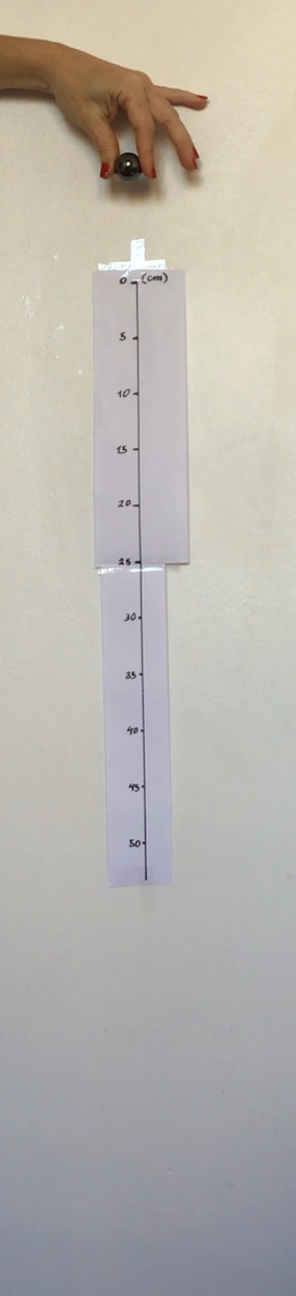
\includegraphics[width=4.5cm]{fig1.pdf}
\label{fig1}
\captionof{figure}{Dispositivo experimental. Não esqueça de colar na parede uma régua de papel, como a indicada na figura, para ser usada como referência na análise de dados.}

\end{minipage}
\clearpage
% ----------------------------------------------------------------------------
\section{Análise de dados}
% ----------------------------------------------------------------------------
\indent 


Usando o aplicativo Tracker ou alternativamente o aplicativo  VidAnalysis, monte a Tabela \ref{tabela1}.
\begin{table}[h!]
\centering
\begin{tabular}{c|c|c|c|c}
t (s) & $y$ (cm) & $\delta y$ (cm)& $v_y$ (cm/s)& $\delta v_y$ (cm/s)\\
\hline 
&&&& 
\end{tabular}
\caption{Tabela de dados da experiência.}
\label{tabela1}
\end{table}
\par
\begin{minipage}[c]{11.5cm}
\hskip 0.5cm
As colunas do tempo $t$ e da posição $y$ são preenchidas usando os aplicativos Tracker 
ou  VidAnalysis. As coordenadas $y$ correspondem às posições, por exemplo, do centro da bolinha ao longo da trajetória de queda, após ter escolhido o sistema de referência. Note que ao longo da trajetória a imagem da bolinha pode ficar um pouco embaçada como na figura ao lado. 
Nesse caso, foi marcado com um "x"  em azul 
o centro da bolinha enquanto que a barra vermelha é uma escolha razoável da região de incerteza
da posição do centro da bolinha.  
\par
\hskip 0.5cm
Para preencher a coluna da velocidade $v_y$ leia o Apêndice \ref{ApendiceD}. 
Como são calculadas as incertezas $\delta v_y$?
\par 
%\hskip 0.5cm
\begin{itemize}
\item Em papel milimetrado desenhe o gráfico $v_y$ vs. $t$ a partir dos dados da tabela indicando 
a incerteza nos valores das velocidades. Qual é a forma esperada para este gráfico?
\item Use as colunas $t$, $v_y$ e $\delta v_y$ para  calcular através do Método dos Mínimos Quadrados (Capítulo 4 da apostila de conceitos básicos) qual é a melhor reta que aproxima os dados experimentais do gráfico $v_y$ vs. $t$. 
\end{itemize}
\end{minipage}
\hskip 0.2cm
\begin{minipage}[c]{6cm}
%%%%%%%%%%%%%%%%%%%%%%%%%%%%%%%%
%\begin{figure}[h!]
%\centering
\hskip 1cm
\includegraphics[width=3.8cm]{fig2.pdf}
\label{fig2}
\captionof{figure}{Imagem da bolinha em plena queda. Note-se que a imagem, devido à alta velocidade, fica um pouco embaçada.}
%\end{figure}
%%%%%%%%%%%%%%%%%%%%%%%%%%%%%%%%
\end{minipage}
\begin{itemize}
\item Com os parâmetros da reta obtida no item anterior,  desenhe ela  na mesma folha milimetrada 
que fez o gráfico $v_y$ vs. $t$. Se você não conseguir um aplicativo que implemente o ajuste linear pelo método dos mínimos quadrados desenhe a melhor reta que aproxima os dados experimentais 
pelo método visual (ver o Apêndice \ref{ApendiceG}) e obtenha os parâmetros que definem a reta 
(inclinação $a$ e coeficiente linear $b$) escolhendo dois pontos na reta e substituindo na equação da reta $y=a\;t+b$.
\end{itemize}
  
\clearpage

% ----------------------------------------------------------------------------
\section{Discussão dos resultados}
% ----------------------------------------------------------------------------

\begin{enumerate}
\item A partir dos parâmetros do ajuste linear aos dados experimentais $v_y$ vs. $t$, 
como se obtêm o valor da aceleração de queda da bolinha?
\item 
Compare o valor da aceleração de queda da bolinha com o valor da aceleração da gravidade 
para a cidade do Rio de Janeiro que é $g=(978,7\pm 0.1) cm/s^2)$. 
Qual valor é mais preciso? Você utilizaria este método para determinar o valor da gravidade? Justifique.
\end{enumerate}
\par 
No relatório você deverá entregar um arquivo pdf que
contenha o objetivo do experimento, a Tabela \ref{tabela1} e o gráfico em papel milimetrado dos dados experimentais de $v_y$ vs. $t$ assim como o ajuste linear. Também deverá entregar nesse arquivo pdf  a discussão dos ítens 1 e 2 acima. 

\section{Opcional: Estudo da conservação da energia}
\indent

Também poderá entregar no arquivo pdf do relatório as seguintes tarefas opcionais:

\begin{enumerate}
\item Utilizando os dados registrados para a posição $y$ como função do tempo $t$, determine a altura $h$ da bolinha para cada instante de tempo, a partir do ponto mais baixo na Tabela \ref{tabela1}.
\item Determine a energia cinética ($K$), energia potencial ($U$) e a energia mecânica ($E$) para cada intervalo de tempo. Para facilitar a organização das informações, construa uma tabela.
\item Faça um gráfico que contenha a energia cinética, potencial e mecânica em função do tempo.
\item Discuta a partir do gráfico obtido, se há ou não conservação da energia mecânica. Justificar.
\item No caso da energia não se conservar, determine o ganho ou perda percentual.
\end{enumerate}
\underline{\bf Observações:}
\\
\begin{itemize}
\item Para os cálculos de energia considere a aceleração da gravidade no Rio de Janeiro, 
sendo $g=(978,7\pm 0.1) cm/s^2)$.
\item Não esqueça de colocar todos os cálculos de propagação de incerteza num Apêndice.
\end{itemize}

\clearpage

\appendix
 %-----------------------------------------------------------------------------------------------------------------
\section{Apêndice A: Movimento Retilíneo Uniformemente Variado (MRUV)}
\label{ApendiceA}
 %-----------------------------------------------------------------------------------------------------------------
\indent

Se a força resultante sobre uma partícula de massa $m$ for, $\vec{F}$, a  segunda lei de Newton diz que:
\beq
\label{eqA1}
\vec{F}=m\vec{a},
\eeq
com $\vec{a}$ sendo o vetor aceleração da partícula. No caso de $\vec{F}$ ser uma força constante,
{\it viz.} não depende nem do tempo, nem da posição da partícula e nem da velocidade da mesma, da Eq.(\ref{eqA1}) vemos que 
a aceleração $\vec{a}$ é constante. Assim, a Eq.(\ref{eqA1}) pode ser facilmente integrada para obtermos:
\beq
\label{eqA2}
\int_{t_0}^{t}\vec{F}dt=m\int_{t_0}^{t} \vec{a}dt\Longrightarrow \vec{F}(t-t_0)=m(\vec{v}-\vec{v}_0)
\Longrightarrow \vec{v}=\vec{v}_0+\frac{\vec{F}}{m} (t-t_0),
\eeq
com $\vec{v}:=\vec{v}(t)$ e $\vec{v}_0:=\vec{v}(t_0)$.
Integrando temporalmente mais uma vez ambos os membros da Eq.(\ref{eqA2}) obtemos:
\beq
\vec{r}=\vec{r}_0+\vec{v}_0(t-t_0)+\frac{1}{2}\frac{\vec{F}}{m}(t-t_0)^2,
\eeq
com $\vec{r}:=\vec{r}(t)$ sendo a posição da partícula como função do tempo e 
$\vec{r}_0:=\vec{r}(t_0)$ a sua posição inicial.
\par
Vamos supor agora que a força resultante 
$\vec{F}$ é paralela à velocidade inicial $\vec{v}_0$. Como a soma vetorial de vetores paralelos 
continua sendo um vetor na mesma direção que os vetores somados, de acordo com a Eq.(\ref{eqA2}), a velocidade $\vec{v}(t)$ é paralela a $\vec{v}_0$ para todo tempo. Portanto trata-se 
de um movimento retilíneo. Como também a aceleração é constante o movimento se denomina 
Movimento Retilíneo Uniformemente Variado (MRUV). Sem perda de generalidade podemos 
chamar de eixo ``$y$'' o eixo coordenado na direção de movimento,  e as equações de movimento,  Eqs.(\ref{eqA1}) e (\ref{eqA2}), nessa direção são:
\bea
y&=&y_0+v_{y0}(t-t_0) +\frac{1}{2} \frac{F}{m}(t_0)^2,\\
v_y&=&v_{y0}+\frac{F}{m}(t-t_0),
\eea 
com $y:=y(t)$ e $v_y:=v_y(t)$ e as condições iniciais, $y_0:=y(t_0)$ e $v_{y0}:=v_y(t_0)$.

\clearpage
%-----------------------------------------------------------------------------------------------------------------
\section{Apêndice B: Tutorial básico de uso do aplicativo Tracker.}
\label{ApendiceB}
 %-----------------------------------------------------------------------------------------------------------------
\indent

Uma vez baixada a versão do aplicativo Tracker para o sistema operacional de seu computador 
desde o endereço eletrônico  {\color{blue} https://physlets.org/tracker/} instale-o seguindo as orientações no próprio sítio em internet. Com o aplicativo instalado siga os passos a seguir para realizar a tomada de dados.


\underline{\bf Passo 1:} {\bf Escolha de idioma português}\\
\indent 

Abra o aplicativo e no caminho Edit$>$Language$>$ e escolha a opção português como mostra a Figura \ref{fig1AppB}.

\begin{figure}[h!]
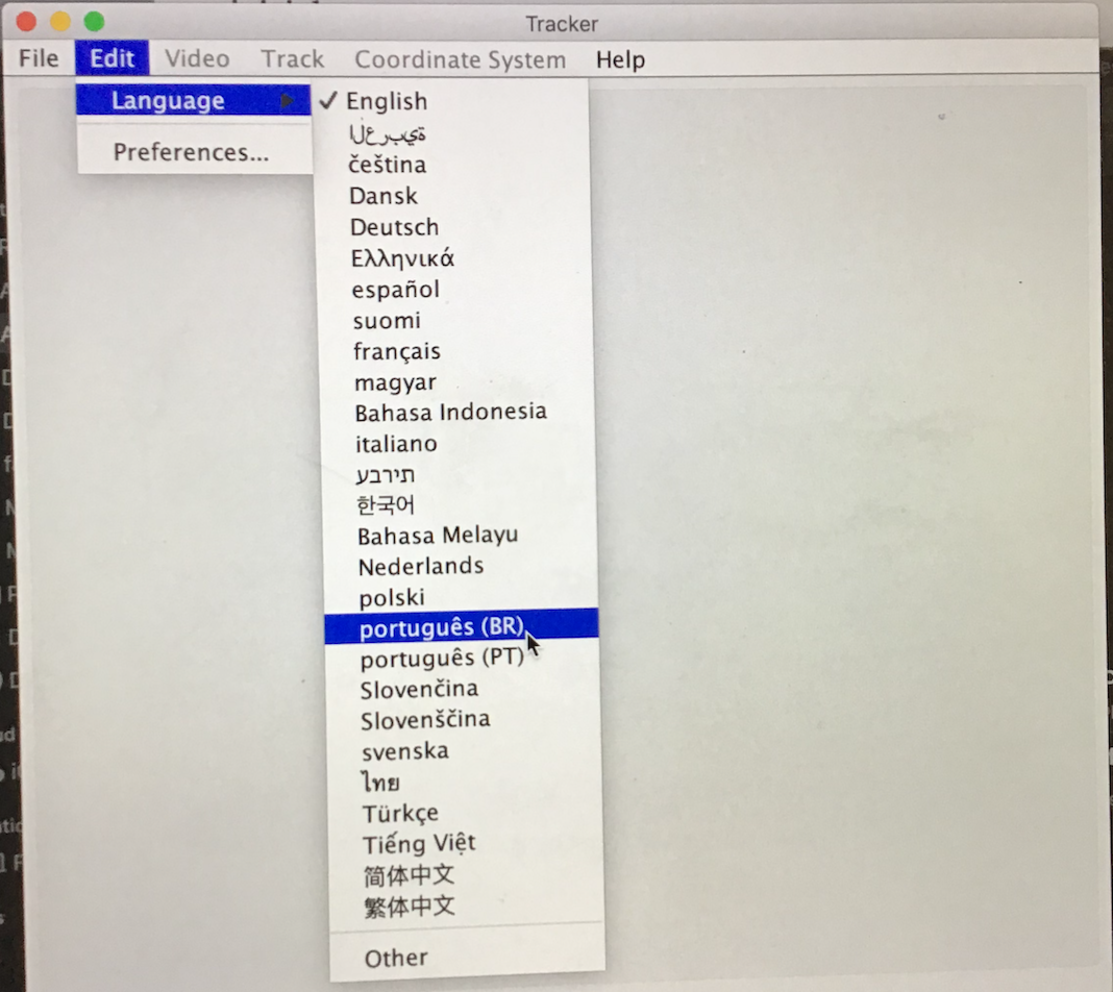
\includegraphics[width=9cm]{fig1AppB.pdf}
\caption{Escolha de idioma no aplicativo Tracker.}
\label{fig1AppB}
\end{figure}

\underline{\bf Passo 2:} {\bf Abertura do arquivo filmico (vídeo) a ser analisado}\\
\indent 

Para abrir o arquivo fílmico gravado com o celular faça um click na aba
``Arquivo'' e logo na aba ``Abrir''. Na janela que abrirá procure onde o arquivo fílmico 
está guardado e faça click nele. O Tracker carrega vídeos de quase todos os formatos gravados 
por celulares mas os arquivos não podem ser muito grandes (o arquivo carregado nas figuras 
deste tutorial era de 1,3 MB). Se o arquivo não abre tente reduzir o tamanho dele editando 
o vídeo no celular, cortando as partes em que a bolinha não se move, antes da queda, ou quando
já está no chão.
Na Figura \ref{fig2AppB} vemos um vídeo já aberto para análise.

\begin{figure}[h!]
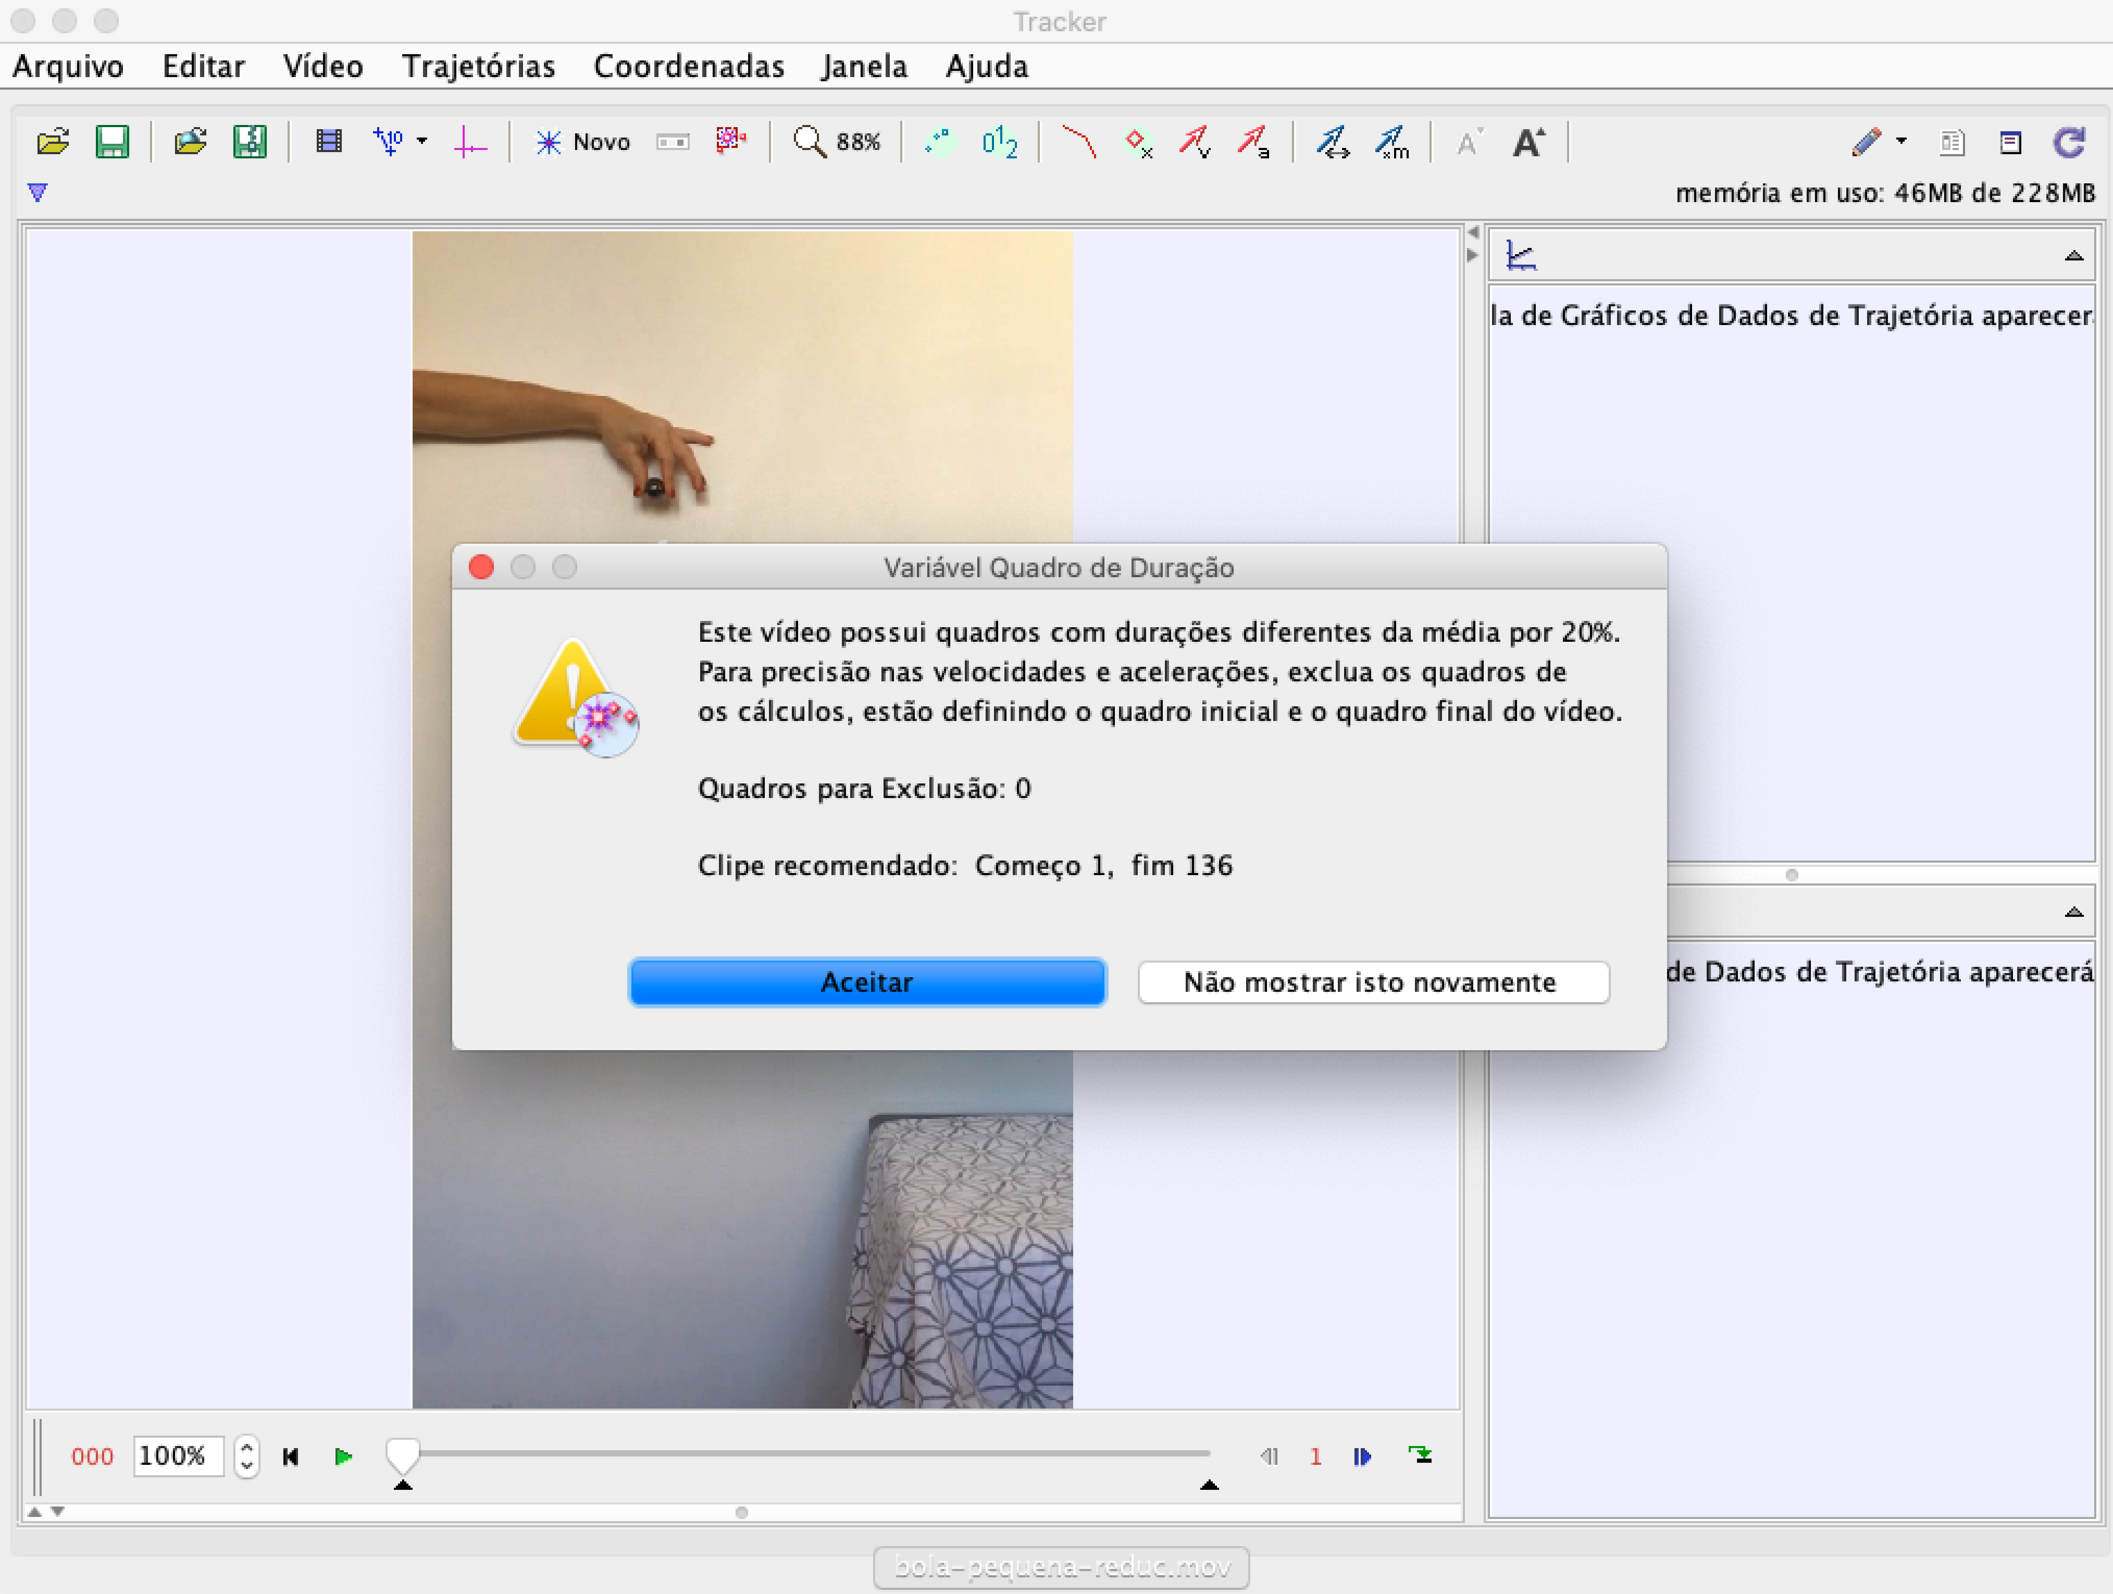
\includegraphics[width=9cm]{fig2AppB.pdf}
\caption{Ignore a mensagem na janela fazendo click em ``Aceitar''.}
\label{fig2AppB}
\end{figure}

\underline{\bf Passo 3:} {\bf Determinação do quadro inicial e final da análise}\\
\indent 

Faça click no ícone indicado pela seta preta na Figura \ref{fig3AppB} para abrir a janela de 
``Ajustes de Corte de Vídeo''. Muitas vezes no lugar assinalado com uma seta vermelha na Figura
\ref{fig3AppB} aparece um valor muito próximo de $30.00/s$ (trinta quadros por segundo), apague o valor e coloque exatamente  $30.00/s$.
\begin{figure}[h!]
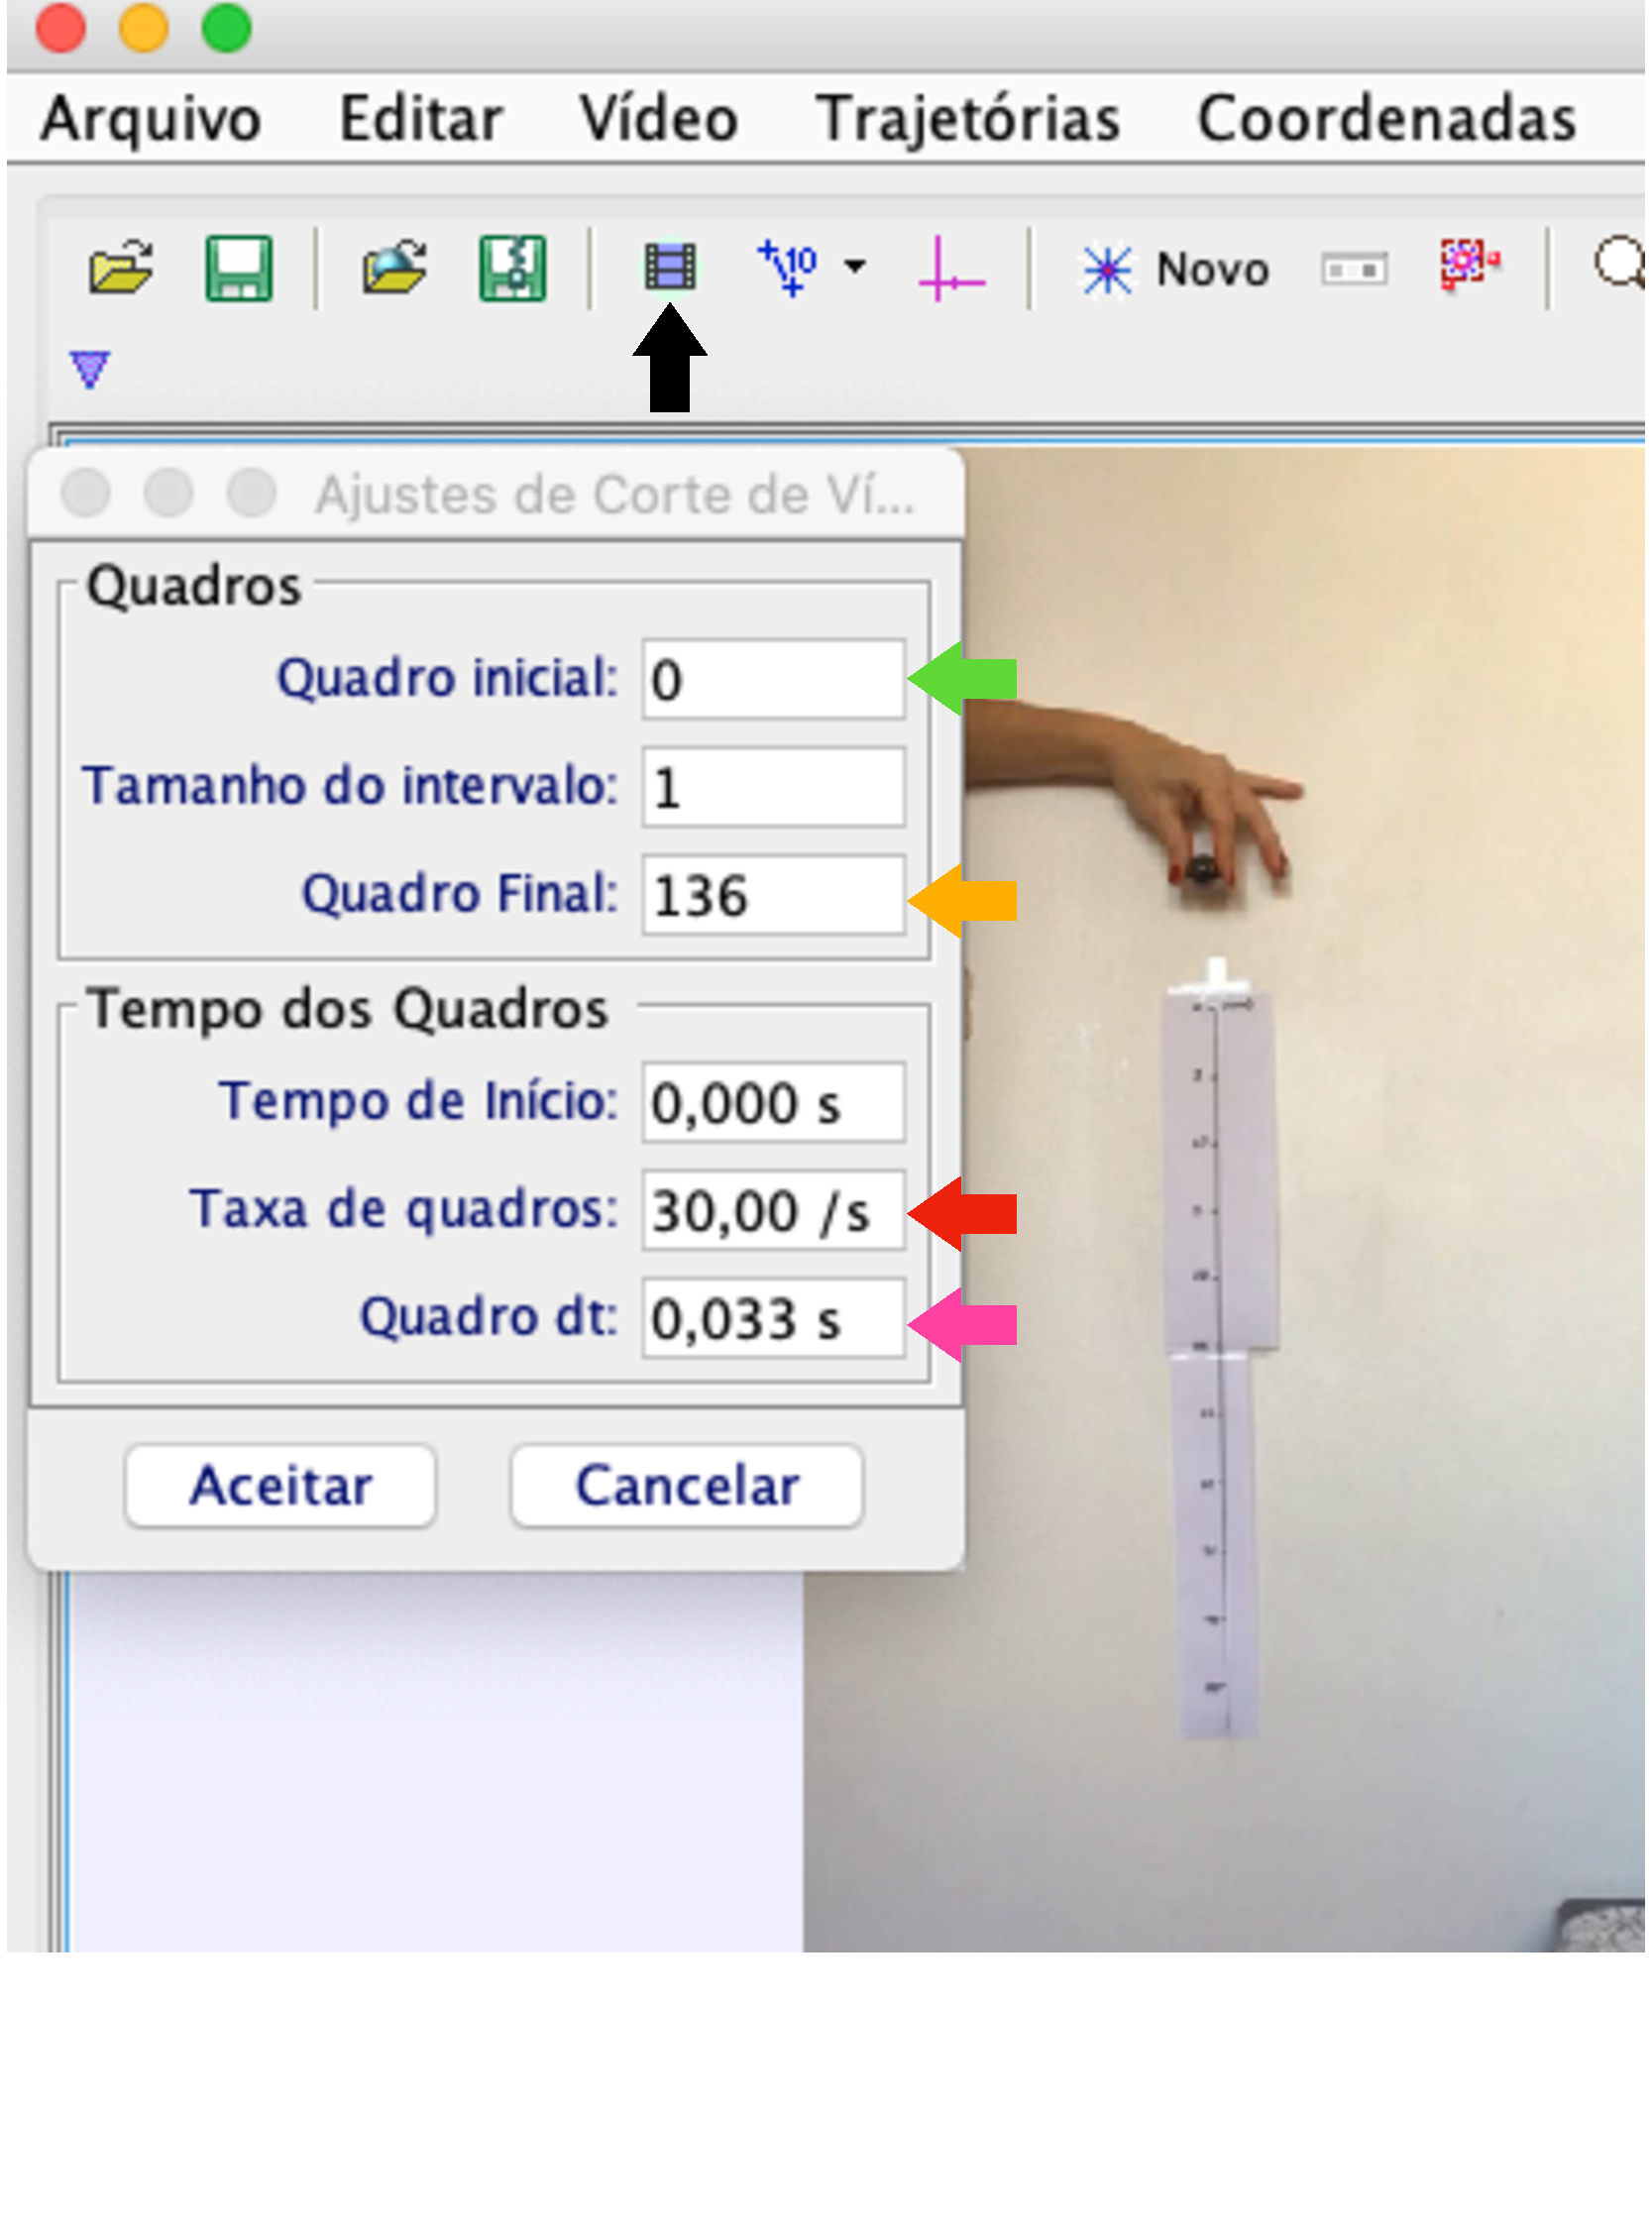
\includegraphics[width=9cm]{fig3AppB.pdf}
\caption{Faça click no ícone indicado pela seta preta para abrir a janela de 
``Ajustes de Corte de Vídeo''.}
\label{fig3AppB}
\end{figure}
As setas verdes e laranja da Figura \ref{fig3AppB} mostram os lugares onde deveremos 
colocar os valores numéricos corretos dos quadros iniciais e finais respectivamente.
Para escolher o quadro inicial correto movimente o ícone preto indicado pela seta verde na Figura 
\ref{fig4AppB} até ver a bolinha justo saindo da mão. Verá que o valor numérico do quadro inicial 
se coloca automaticamente no lugar indicado pela seta verde na Figura \ref{fig3AppB}. Para escolher 
o quadro final faça o mesmo com o ícone preto indicado pela seta laranja na  Figura 
\ref{fig4AppB}. Escolha o quadro final mais o menos como no instante mostrado na  Figura 
\ref{fig4AppB}.
\begin{figure}[h!]
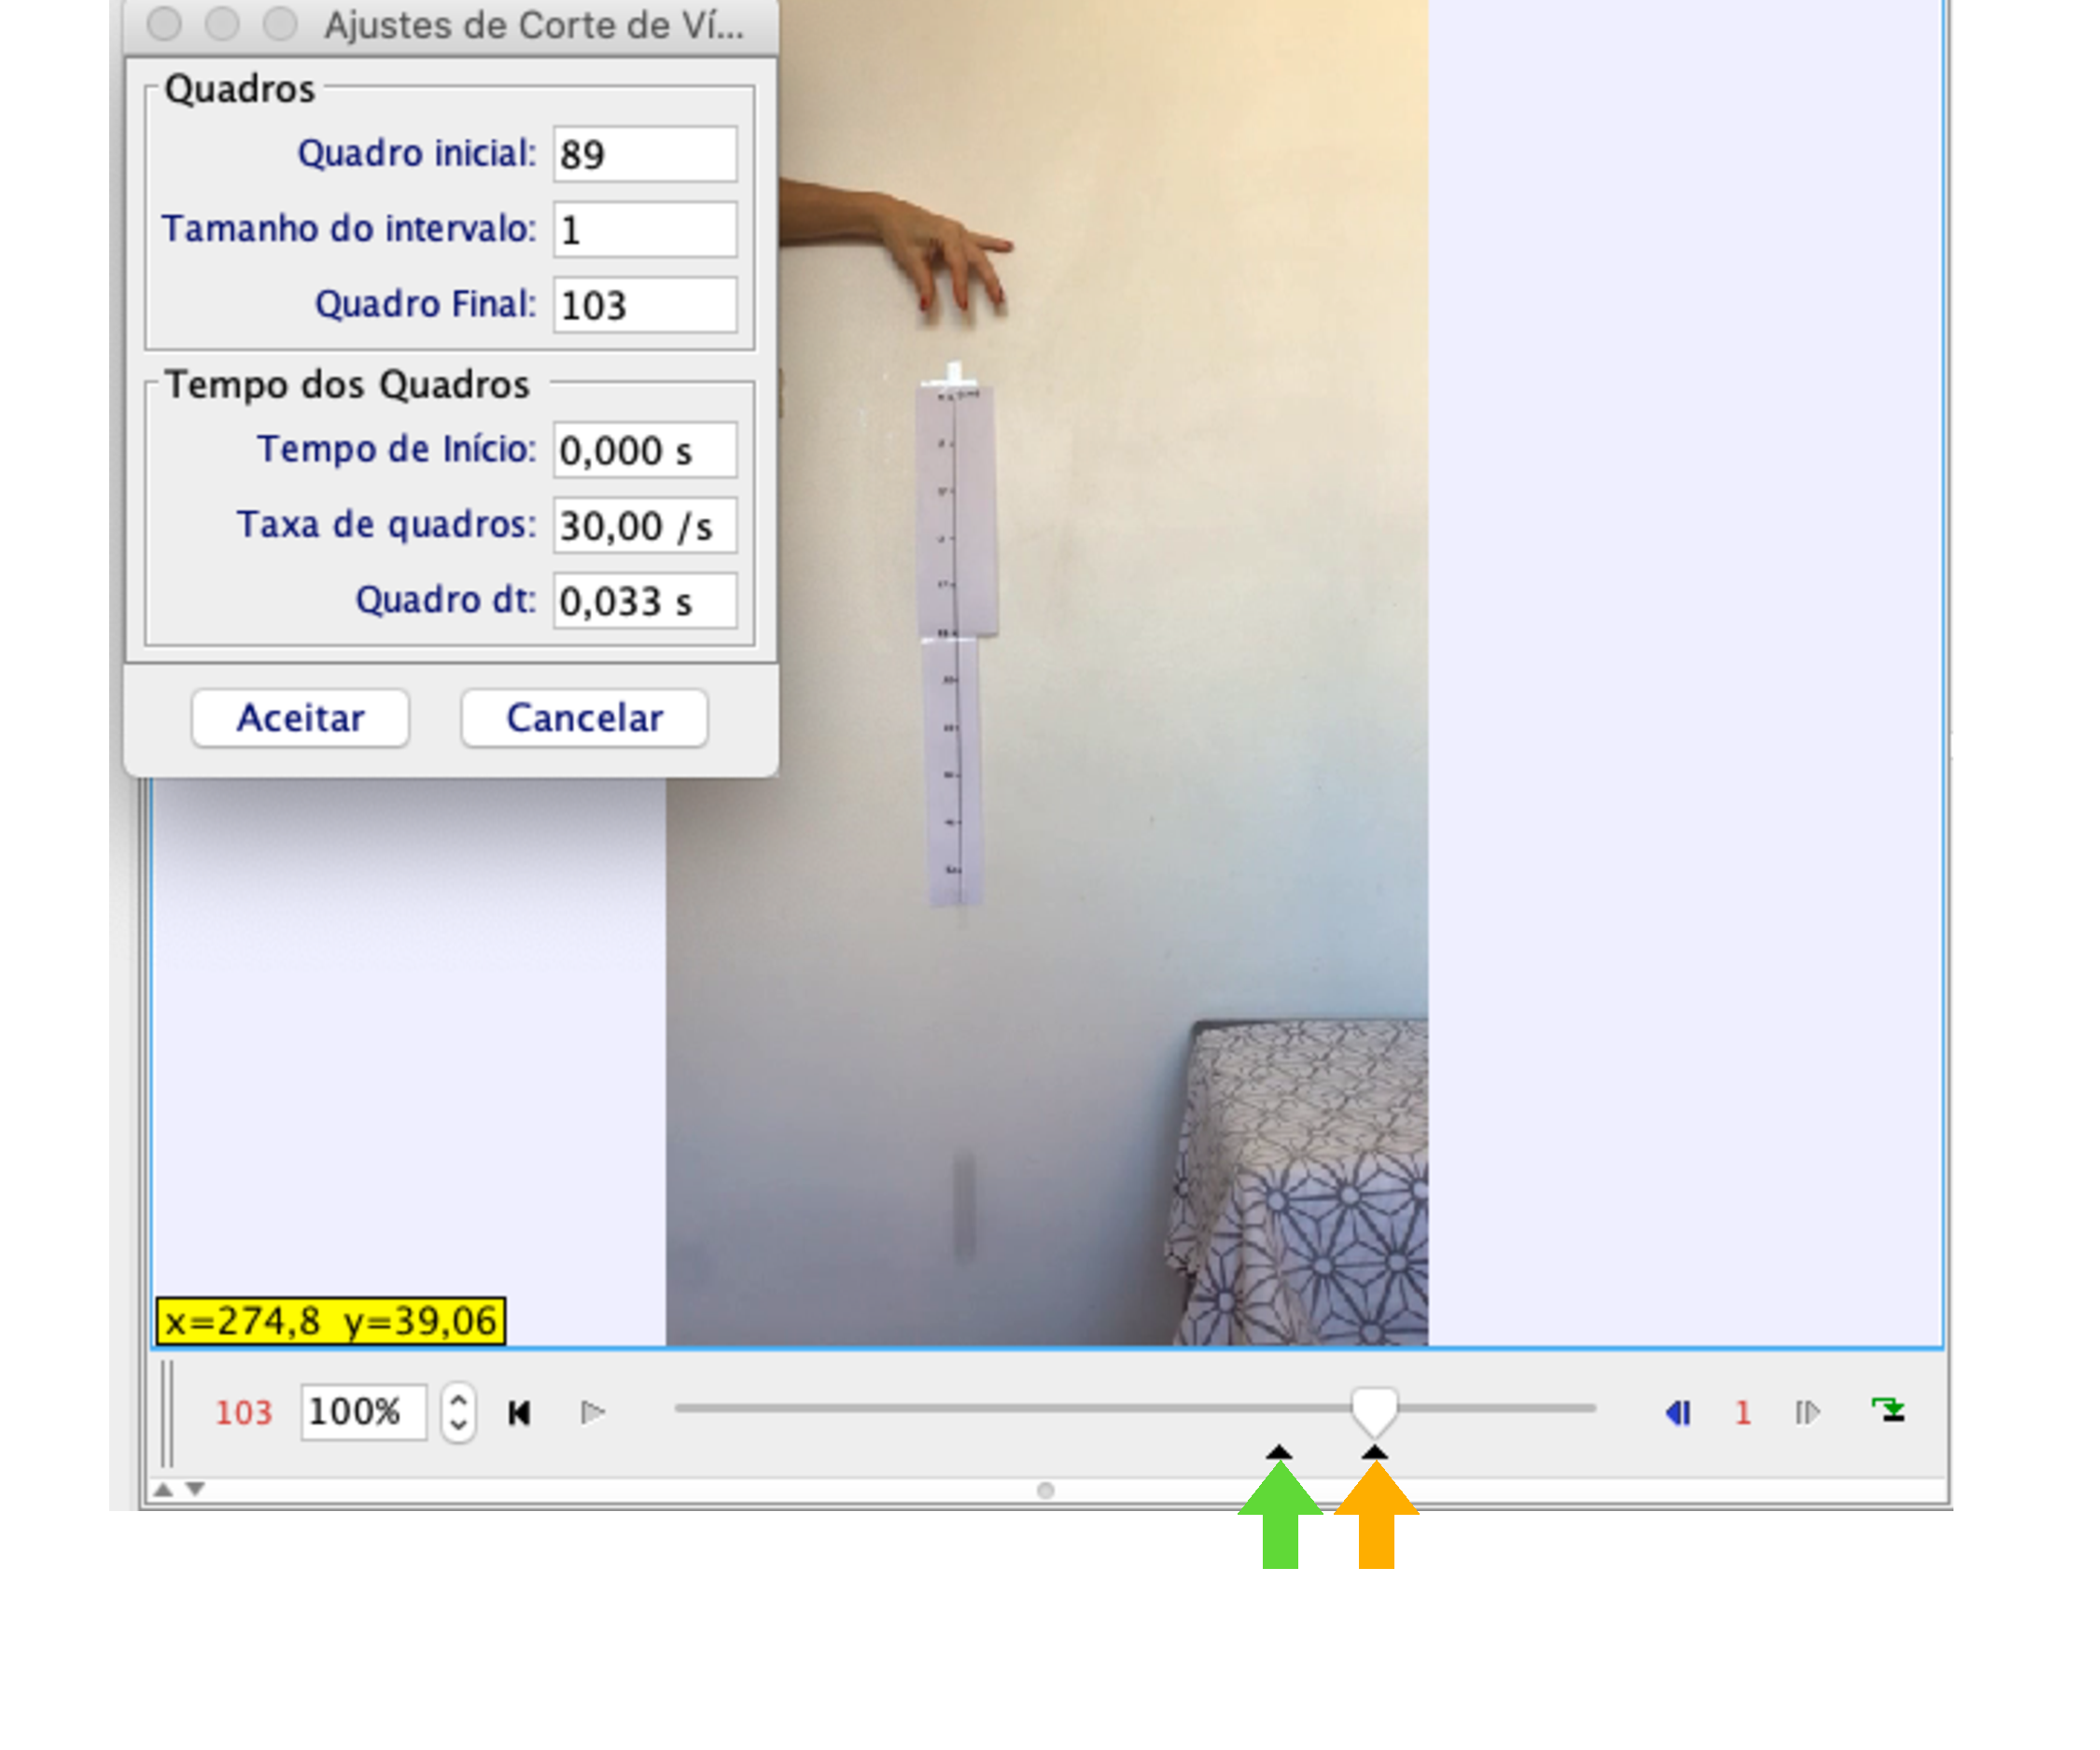
\includegraphics[width=9cm]{fig4AppB.pdf}
\caption{Movimentando os ícones pretos indicados pelas setas verde e laranja escolhemos os quadros iniciais e finais respectivamente.}
\label{fig4AppB}
\end{figure}
Finalmente feche a janela ``Ajustes de Corte de Vídeo'' fazendo click em ``Aceitar''.

\underline{\bf Passo 4:} {\bf Escolha da escala de comprimentos}\\
\indent 

Faça click no ícone indicado pela seta preta  na Figura \ref{fig5AppB} e escolha um novo 
``bastão de medição''. De um ``zoom'' na imagem escolhendo o aumento apropriado no ícone da lupa
de maneira de ver claramente a região da régua na imagem do quadro inicial.  
\begin{figure}[h!]
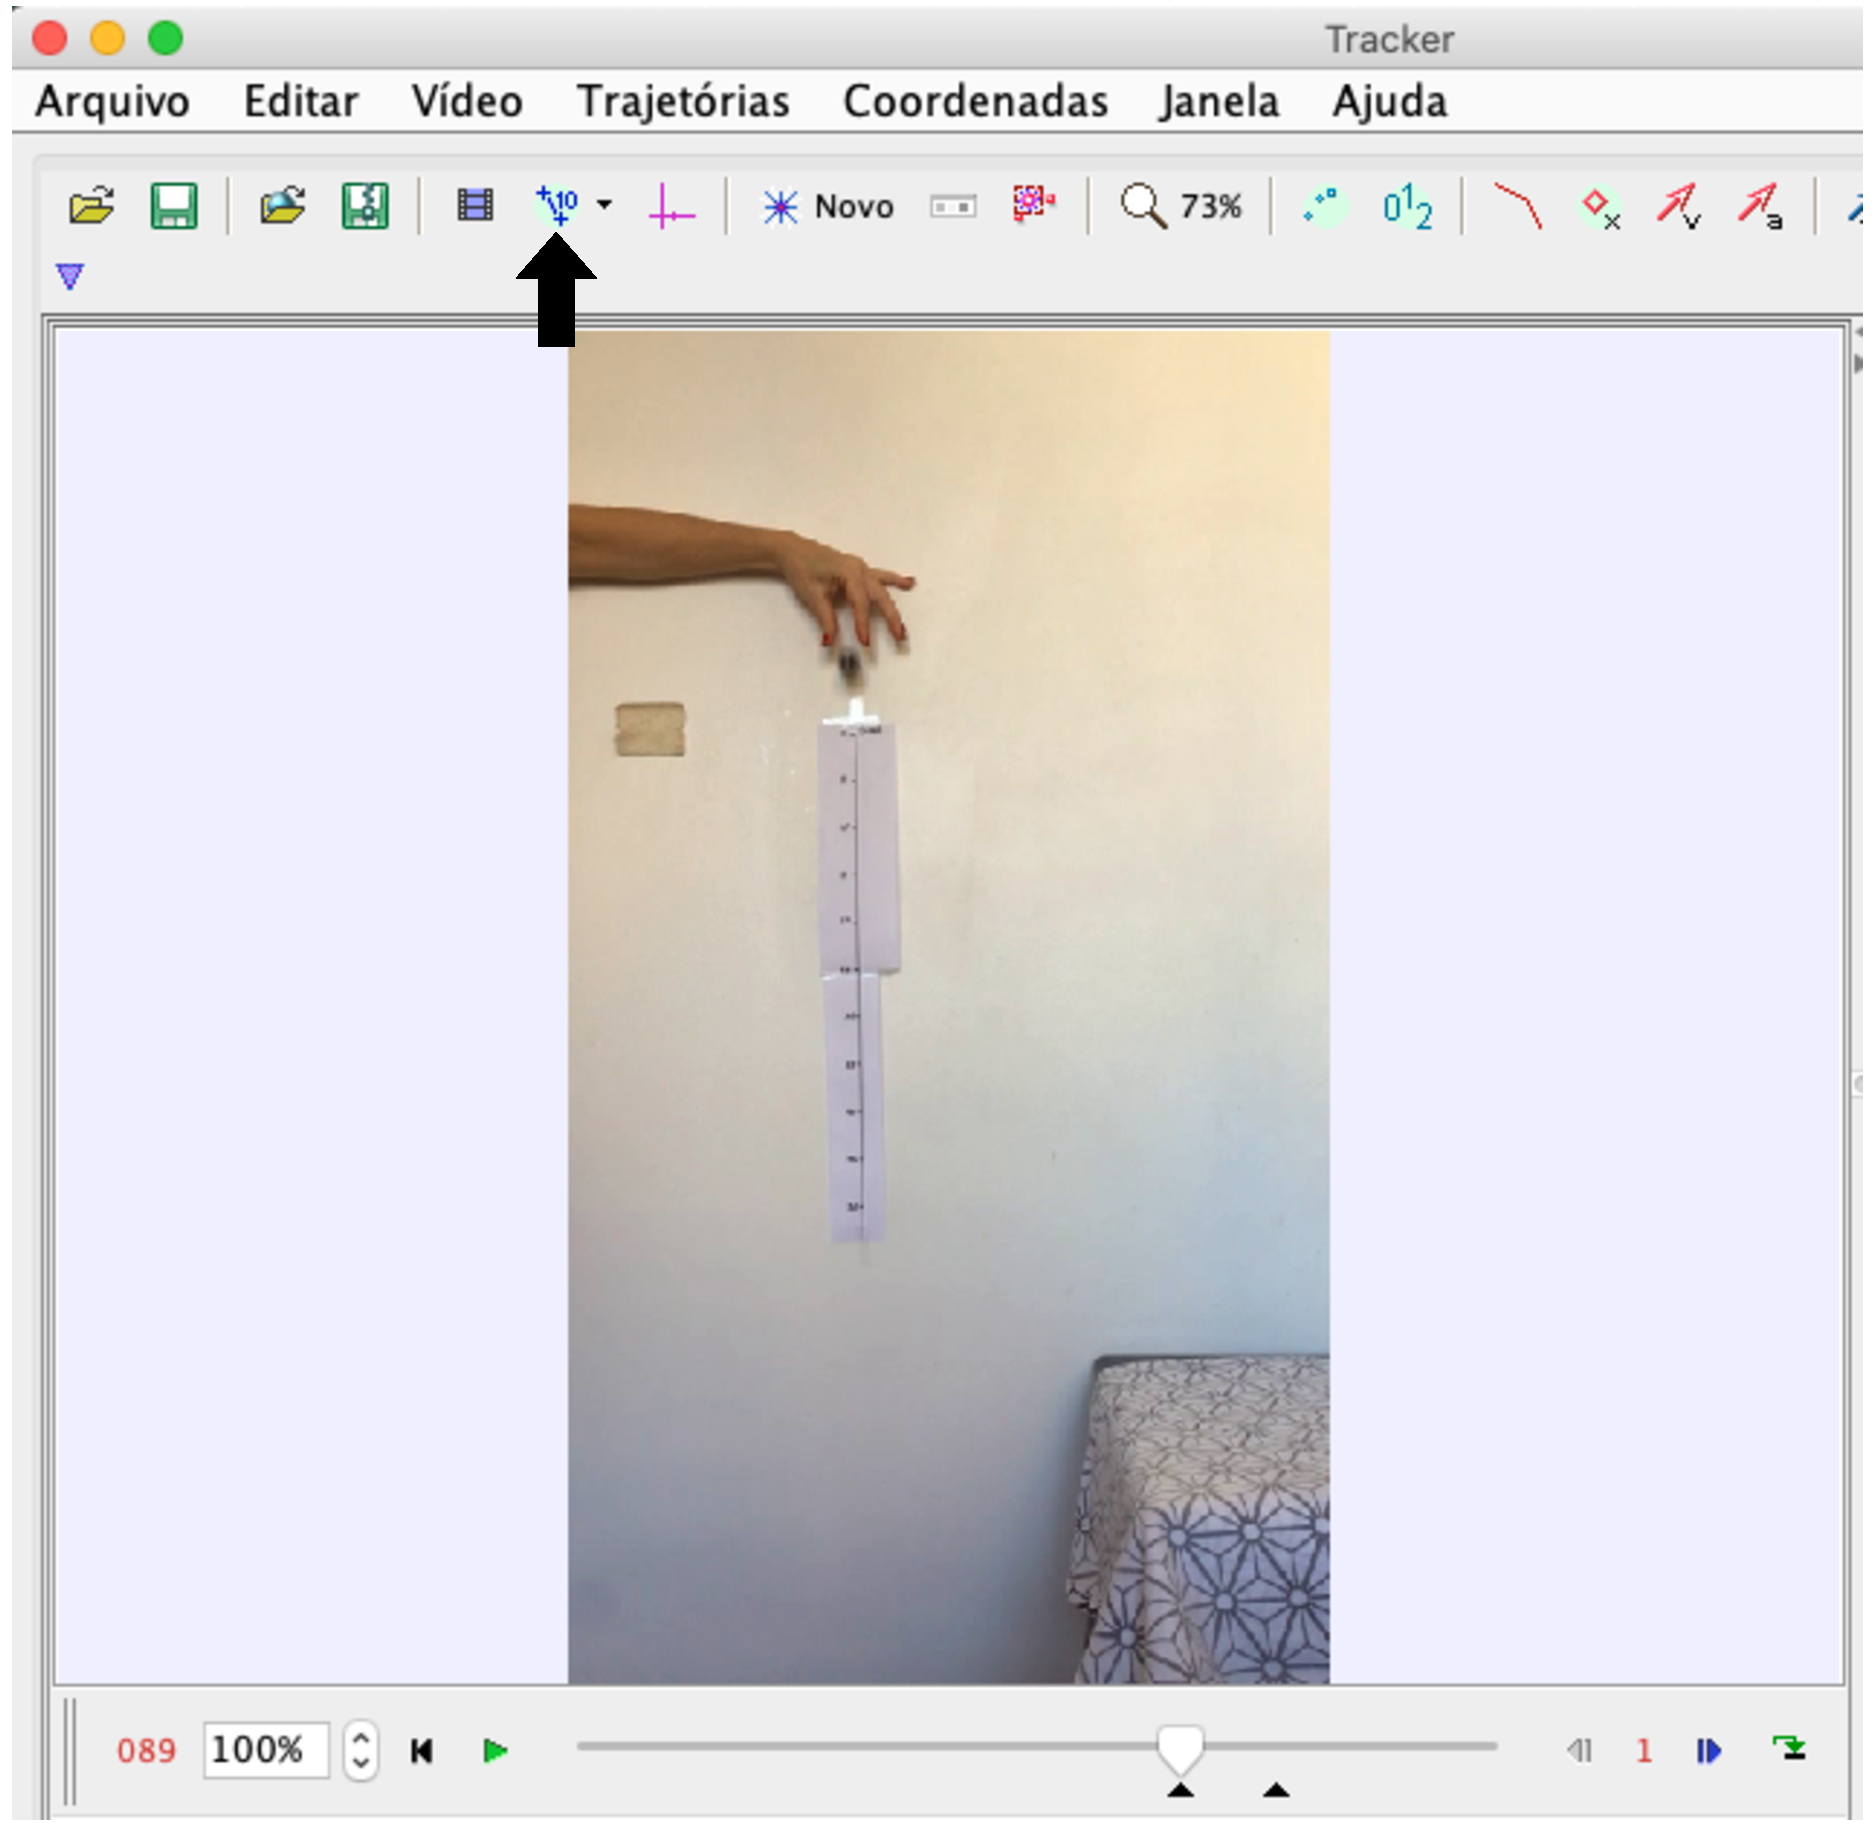
\includegraphics[width=9cm]{fig5AppB.pdf}
\caption{Fazendo click no ícone indicado pela seta preta você pode escolher um ``bastão de medição'' que definirá a escala.}
\label{fig5AppB}
\end{figure}
Mantendo apertada a tecla "shift" do computador selecione os pontos iniciais e finais sobre a régua
como indicado na Figura \ref{fig6AppB}. Não esqueça de colocar na janela indicada nessa figura o valor real do comprimento do ``bastão de medição'' escolhido em metros.
\begin{figure}[h!]
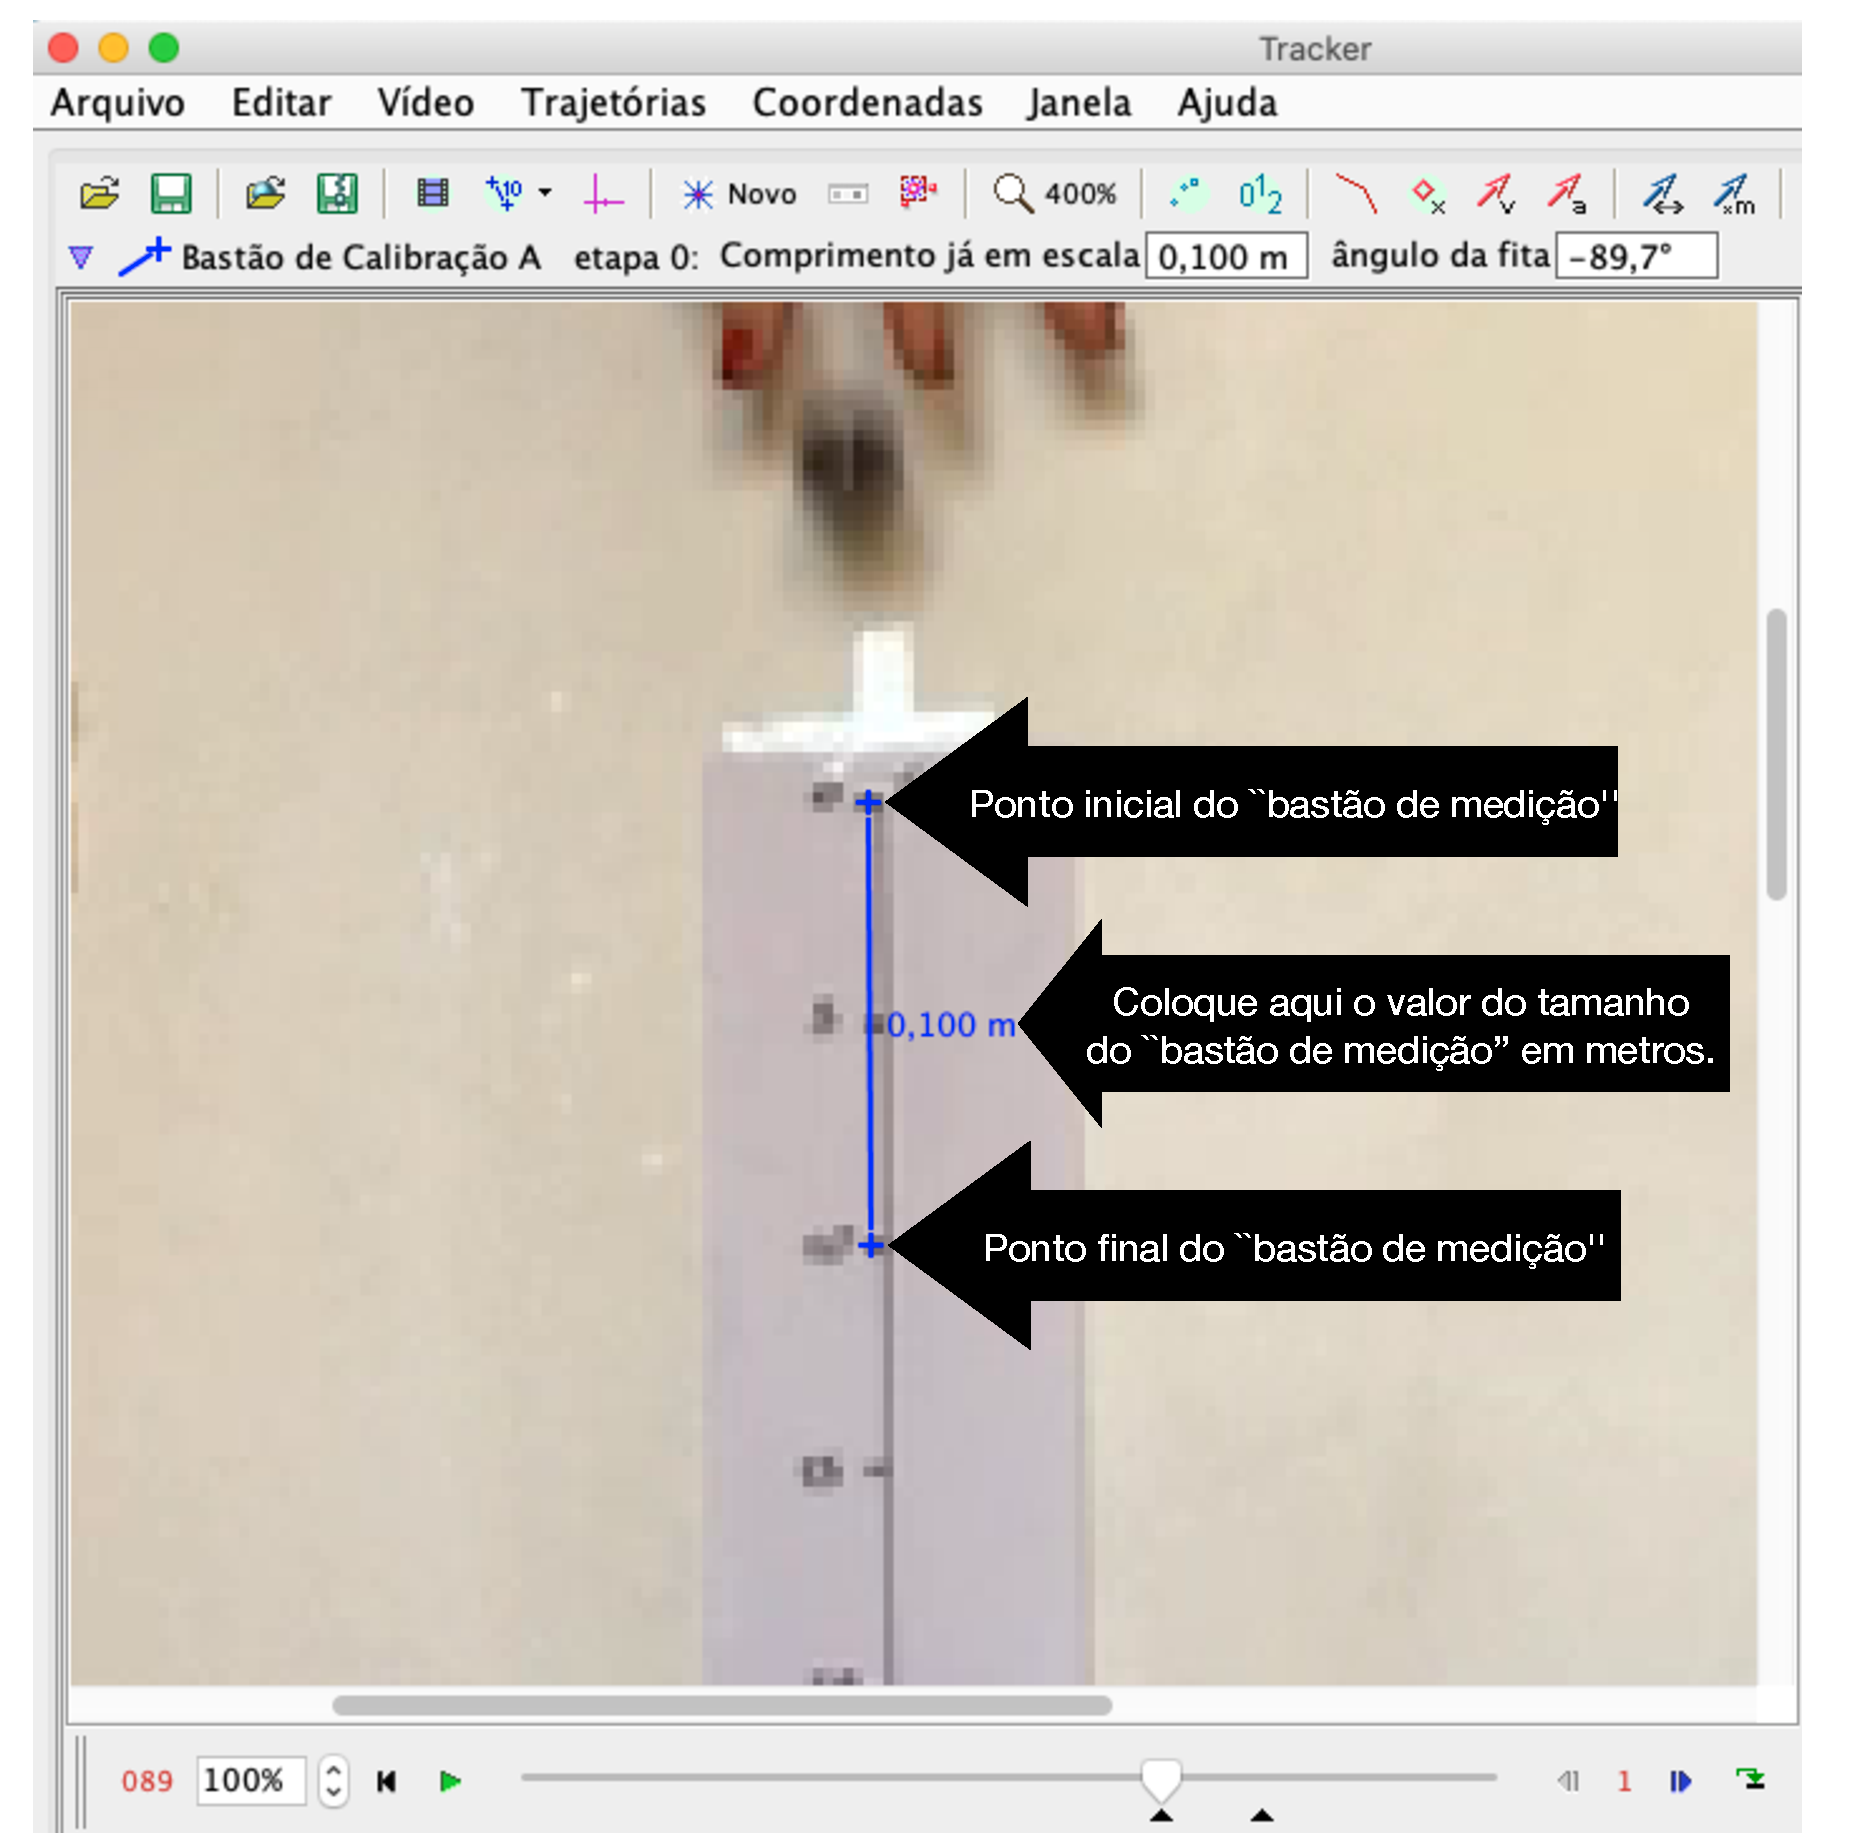
\includegraphics[width=9cm]{fig6AppB.pdf}
\caption{Determinação do ''bastão de medição'' que estabelece a escala de comprimentos.}
\label{fig6AppB}
\end{figure}

\underline{\bf Passo 5:} {\bf Escolha do sistema de coordenadas}\\
\indent

Para escolher um sistema de eixos coordenados faça click no ícone indicado pela seta preta na Figura \ref{fig7AppB}. Dessa forma aparecerá o sistema de eixos cor de rosa da figura. Você pode deslocar 
a origem de coordenadas do sistema de eixos fazendo click com o botão esquerdo do mouse do computador e arrastando a origem para o local que você desejar. Também é possível inclinar o sistema de eixos se for necessário (nesta experiência não será necessário) fazendo click com o botão esquerdo do mouse do computador em qualquer eixo e arrastando esse eixo para obter a inclinação desejada.

\begin{figure}[h!]
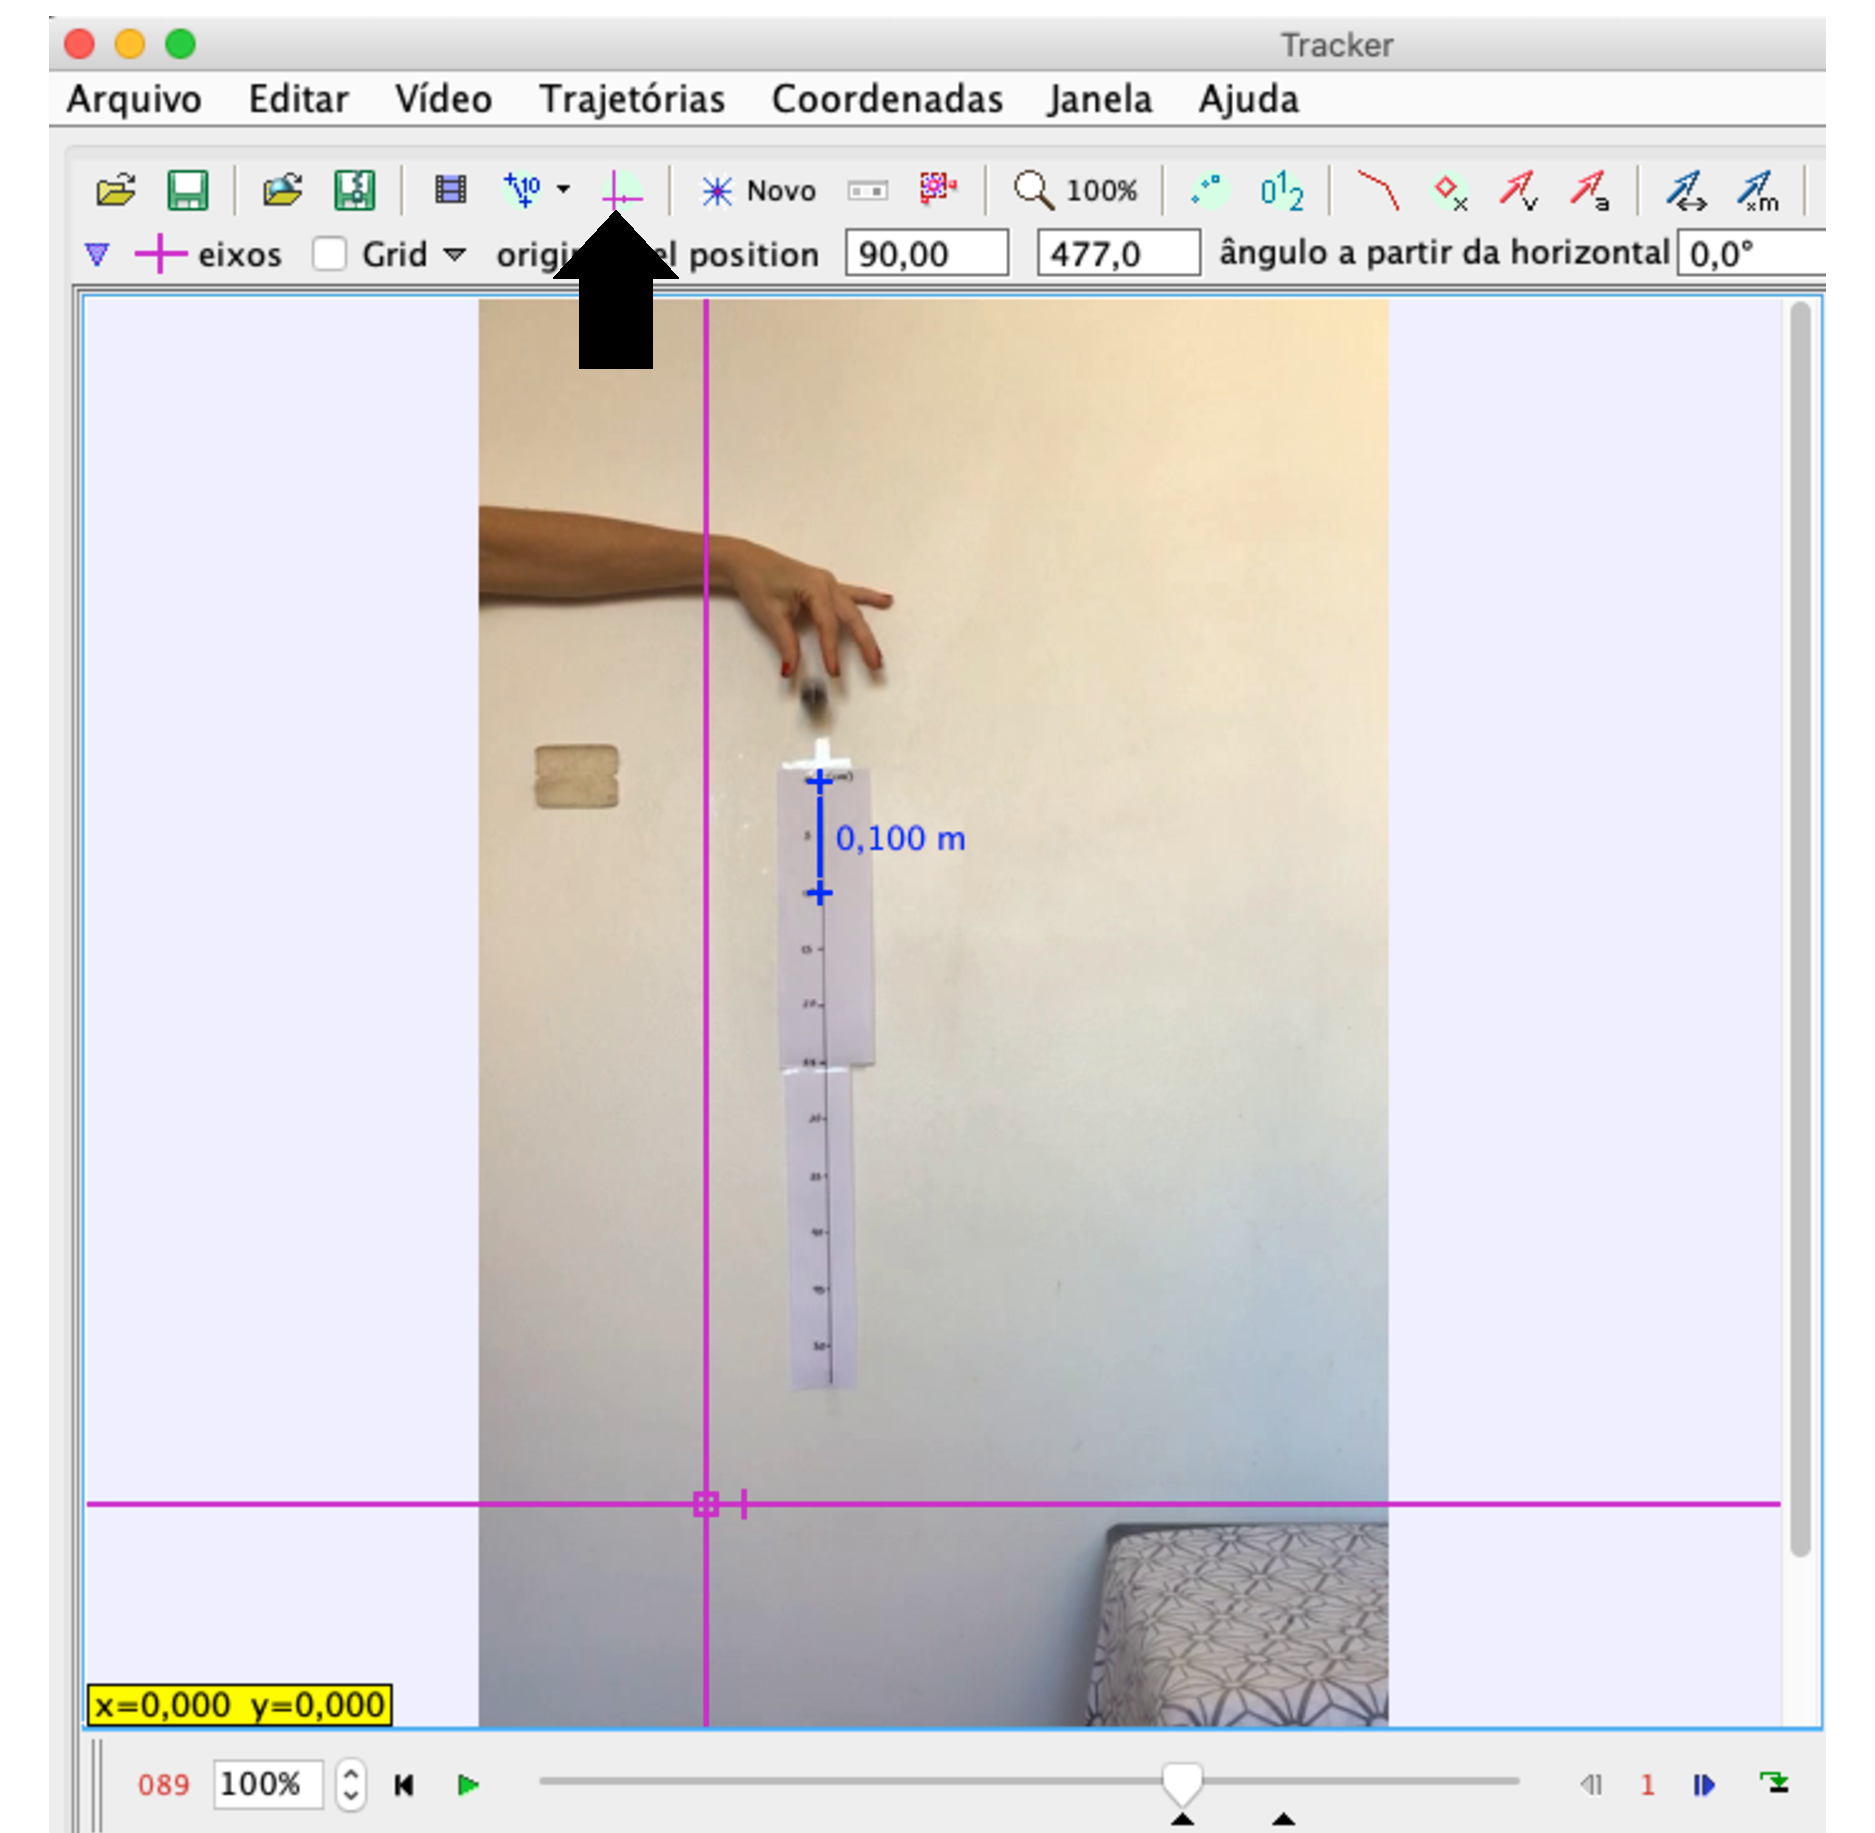
\includegraphics[width=9cm]{fig7AppB.pdf}
\caption{Para criar um sistema de coordenadas (eixos de cor rosa na figura) faça click no ícone indicado pela seta preta. Logo posicione a origem de coordenadas, como mostrado na figura, arrastando com o mouse do computador o quadrado rosa no sistema de eixos.}
\label{fig7AppB}
\end{figure}

\underline{\bf Passo 6:} {\bf Escolha da janela de controle da massa cuja trajetória
será determinada}\\
\indent

Fazendo click no ícone marcado pela seta preta na Figura \ref{fig8AppB} se abrirá a janela de controle 
 da massa (indicada pela seta vermelha  na Figura \ref{fig8AppB}, cuja trajetória será determinada (neste caso a bolinha da figura). Fazendo click na seta verde você poderá escolher qual gráfico 
 quer visualizar uma vez escolhidos os pontos da trajetória cuja forma será ensinada no próximo passo deste tutorial.
\begin{figure}[h!]
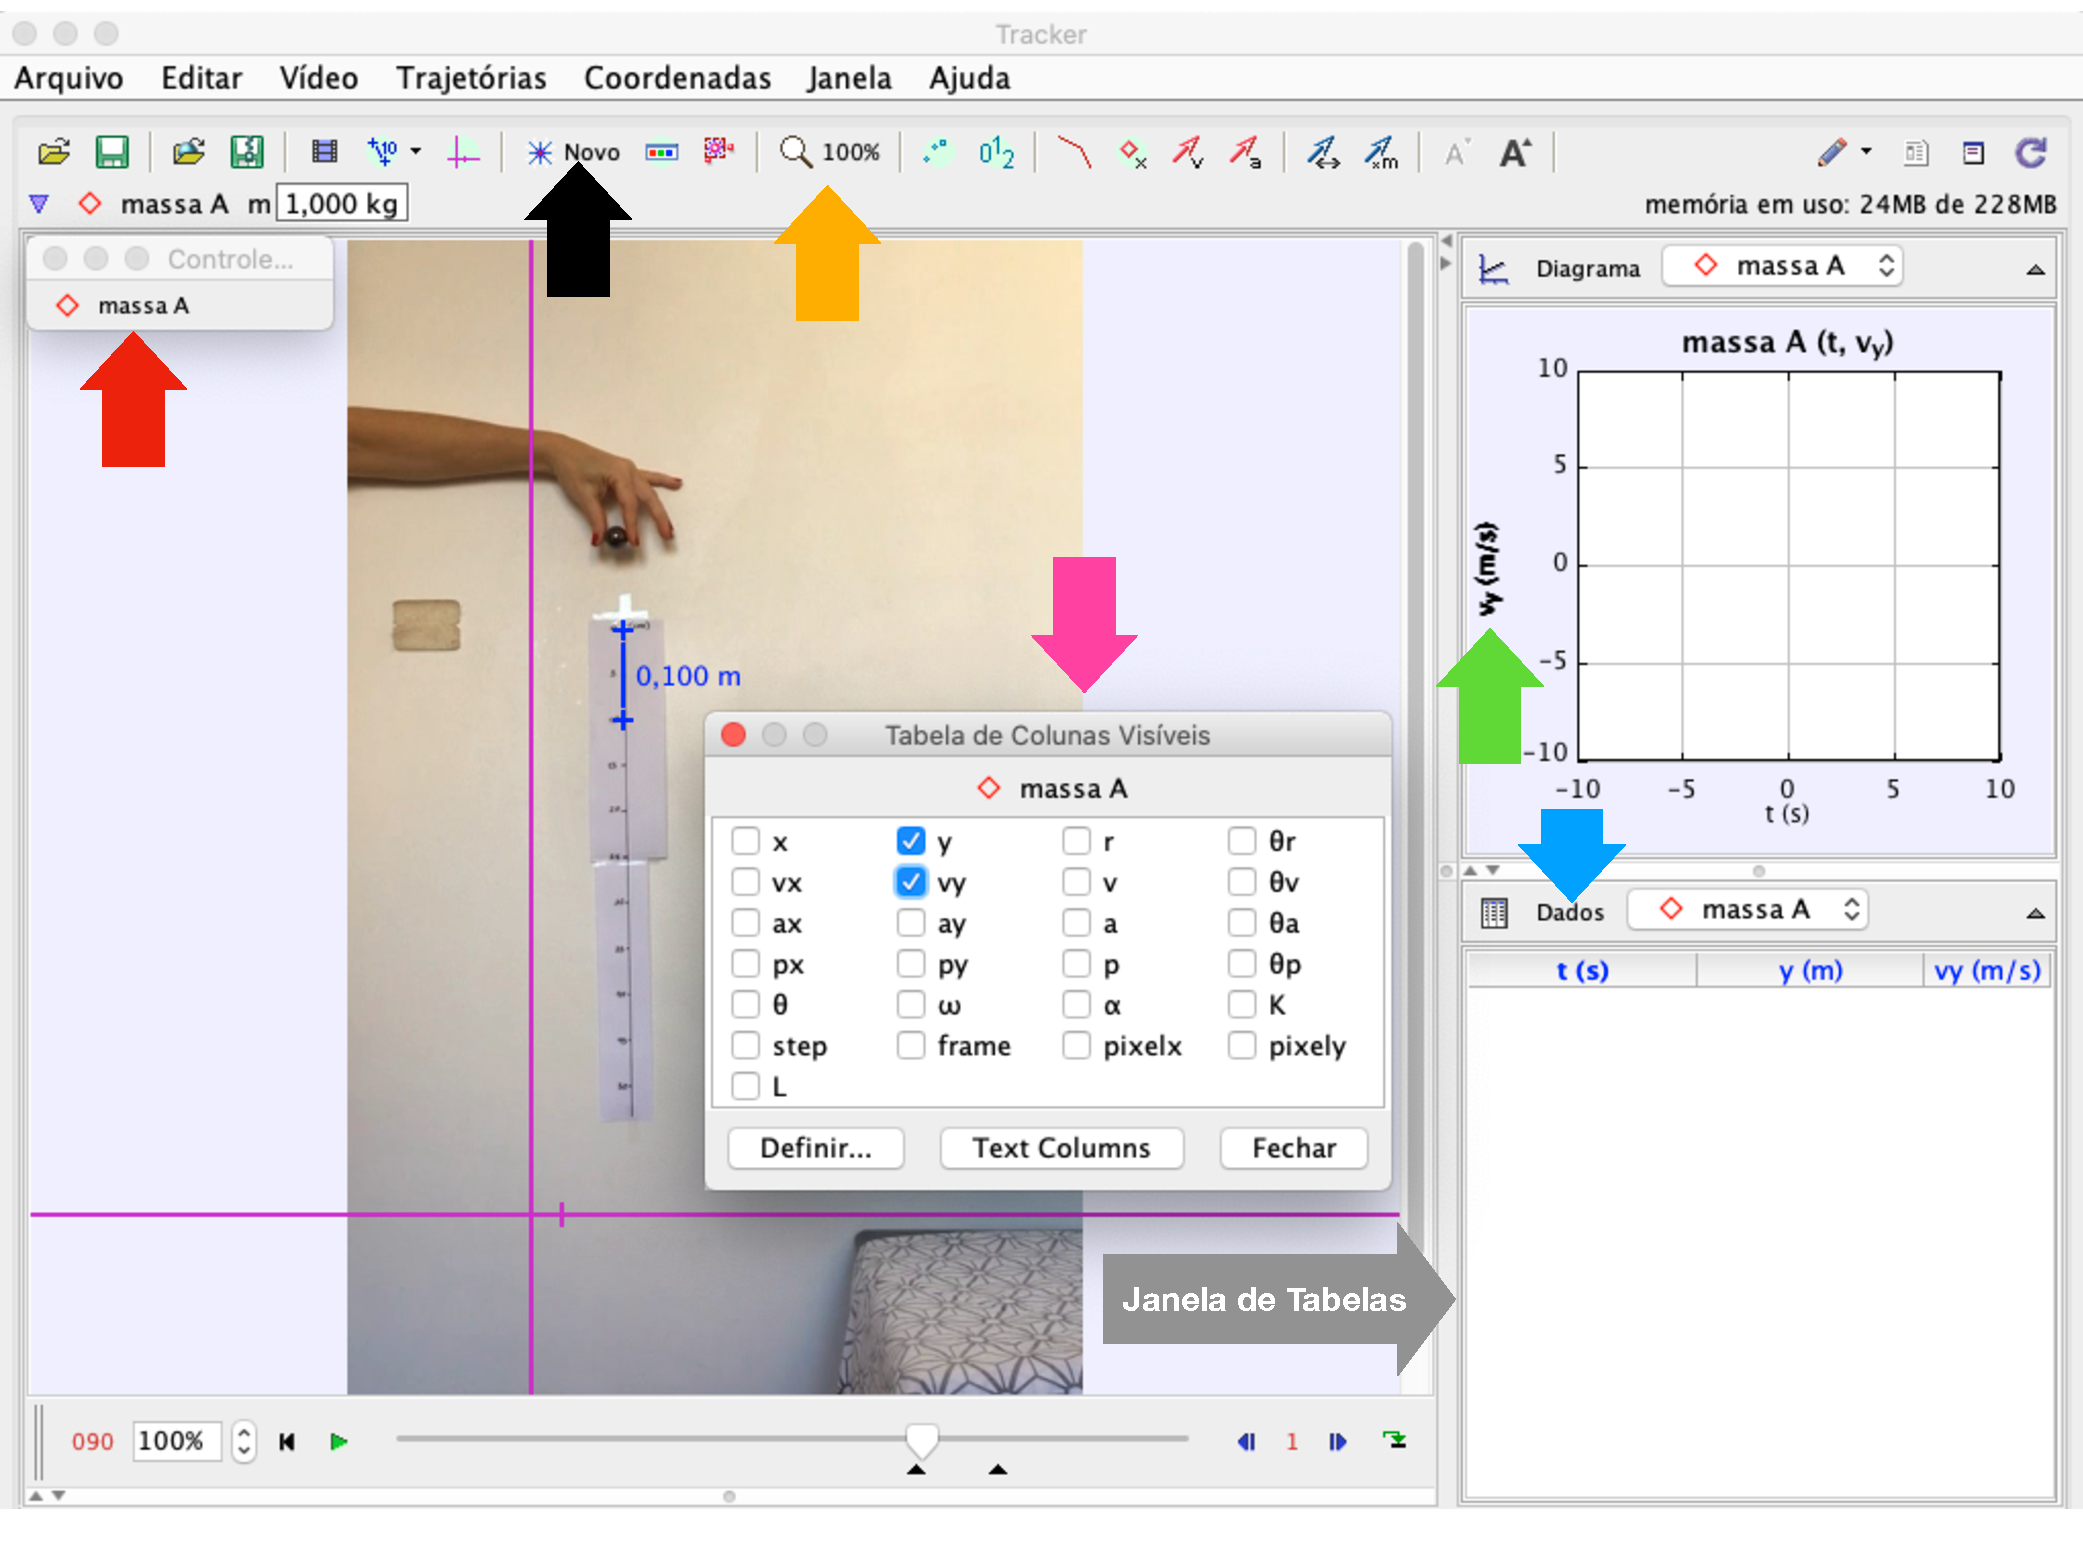
\includegraphics[width=9cm]{fig8AppB.pdf}
\caption{Fazendo click no ícone indicado pela seta preta abre-se a janela indicada pela seta vermelha. Fazendo click no ícone indicado pela seta verde se escolhe o gráfico que quer ser visualizado 
após determinar os pontos da trajetória. Fazendo click na aba ``Dados'', indicada pela seta azul, 
abre-se a janela indicada pela seta rosa onde podem ser escolhidas as colunas das tabelas de dados que apareceram na janela de tabelas. Se precisar fazer um zoom na imagem pode usar a aba indicada pela seta laranja.}
\label{fig8AppB}
\end{figure}
Também fazendo click na aba ``Dados'' assinalada pela seta azul na  Figura \ref{fig8AppB} se abrirá a janela onde você poderá selecionar (seta rosa na figura) as colunas que apareceram na janela de tabelas (indicada também na figura).

\underline{\bf Passo 7:} {\bf Determinação dos pontos da trajetória de uma partícula}\\
\indent

Para determinar os pontos da trajetória em forma manual você precisará manter 
apertada a tecla ``shift'' do computador durante todo o processo de medida . Ao apertar a tecla ``shift'' você entra no modo aquisição de dados e verá que o cursor virá um quadrado com um ``x'' no meio.
Ao fazer click no ponto que você quer traçar a trajetória (no nosso caso será o centro da bolinha)
pela primeira vez se marca um ponto da trajetória e a imagem pula automaticamente para o próximo quadro e ali você pode marcar o centro da bolinha novamente. Repita esse processo até marcar todos os pontos da trajetória contidos nas imagens entre os quadros iniciais e finais determinadas no passo 3 deste tutorial. À medida que você vai marcando os pontos da trajetória as colunas nas tabelas de dados (ver Figura \ref{fig8AppB}) vão sendo preenchidas em forma automática.
\begin{figure}[h!]
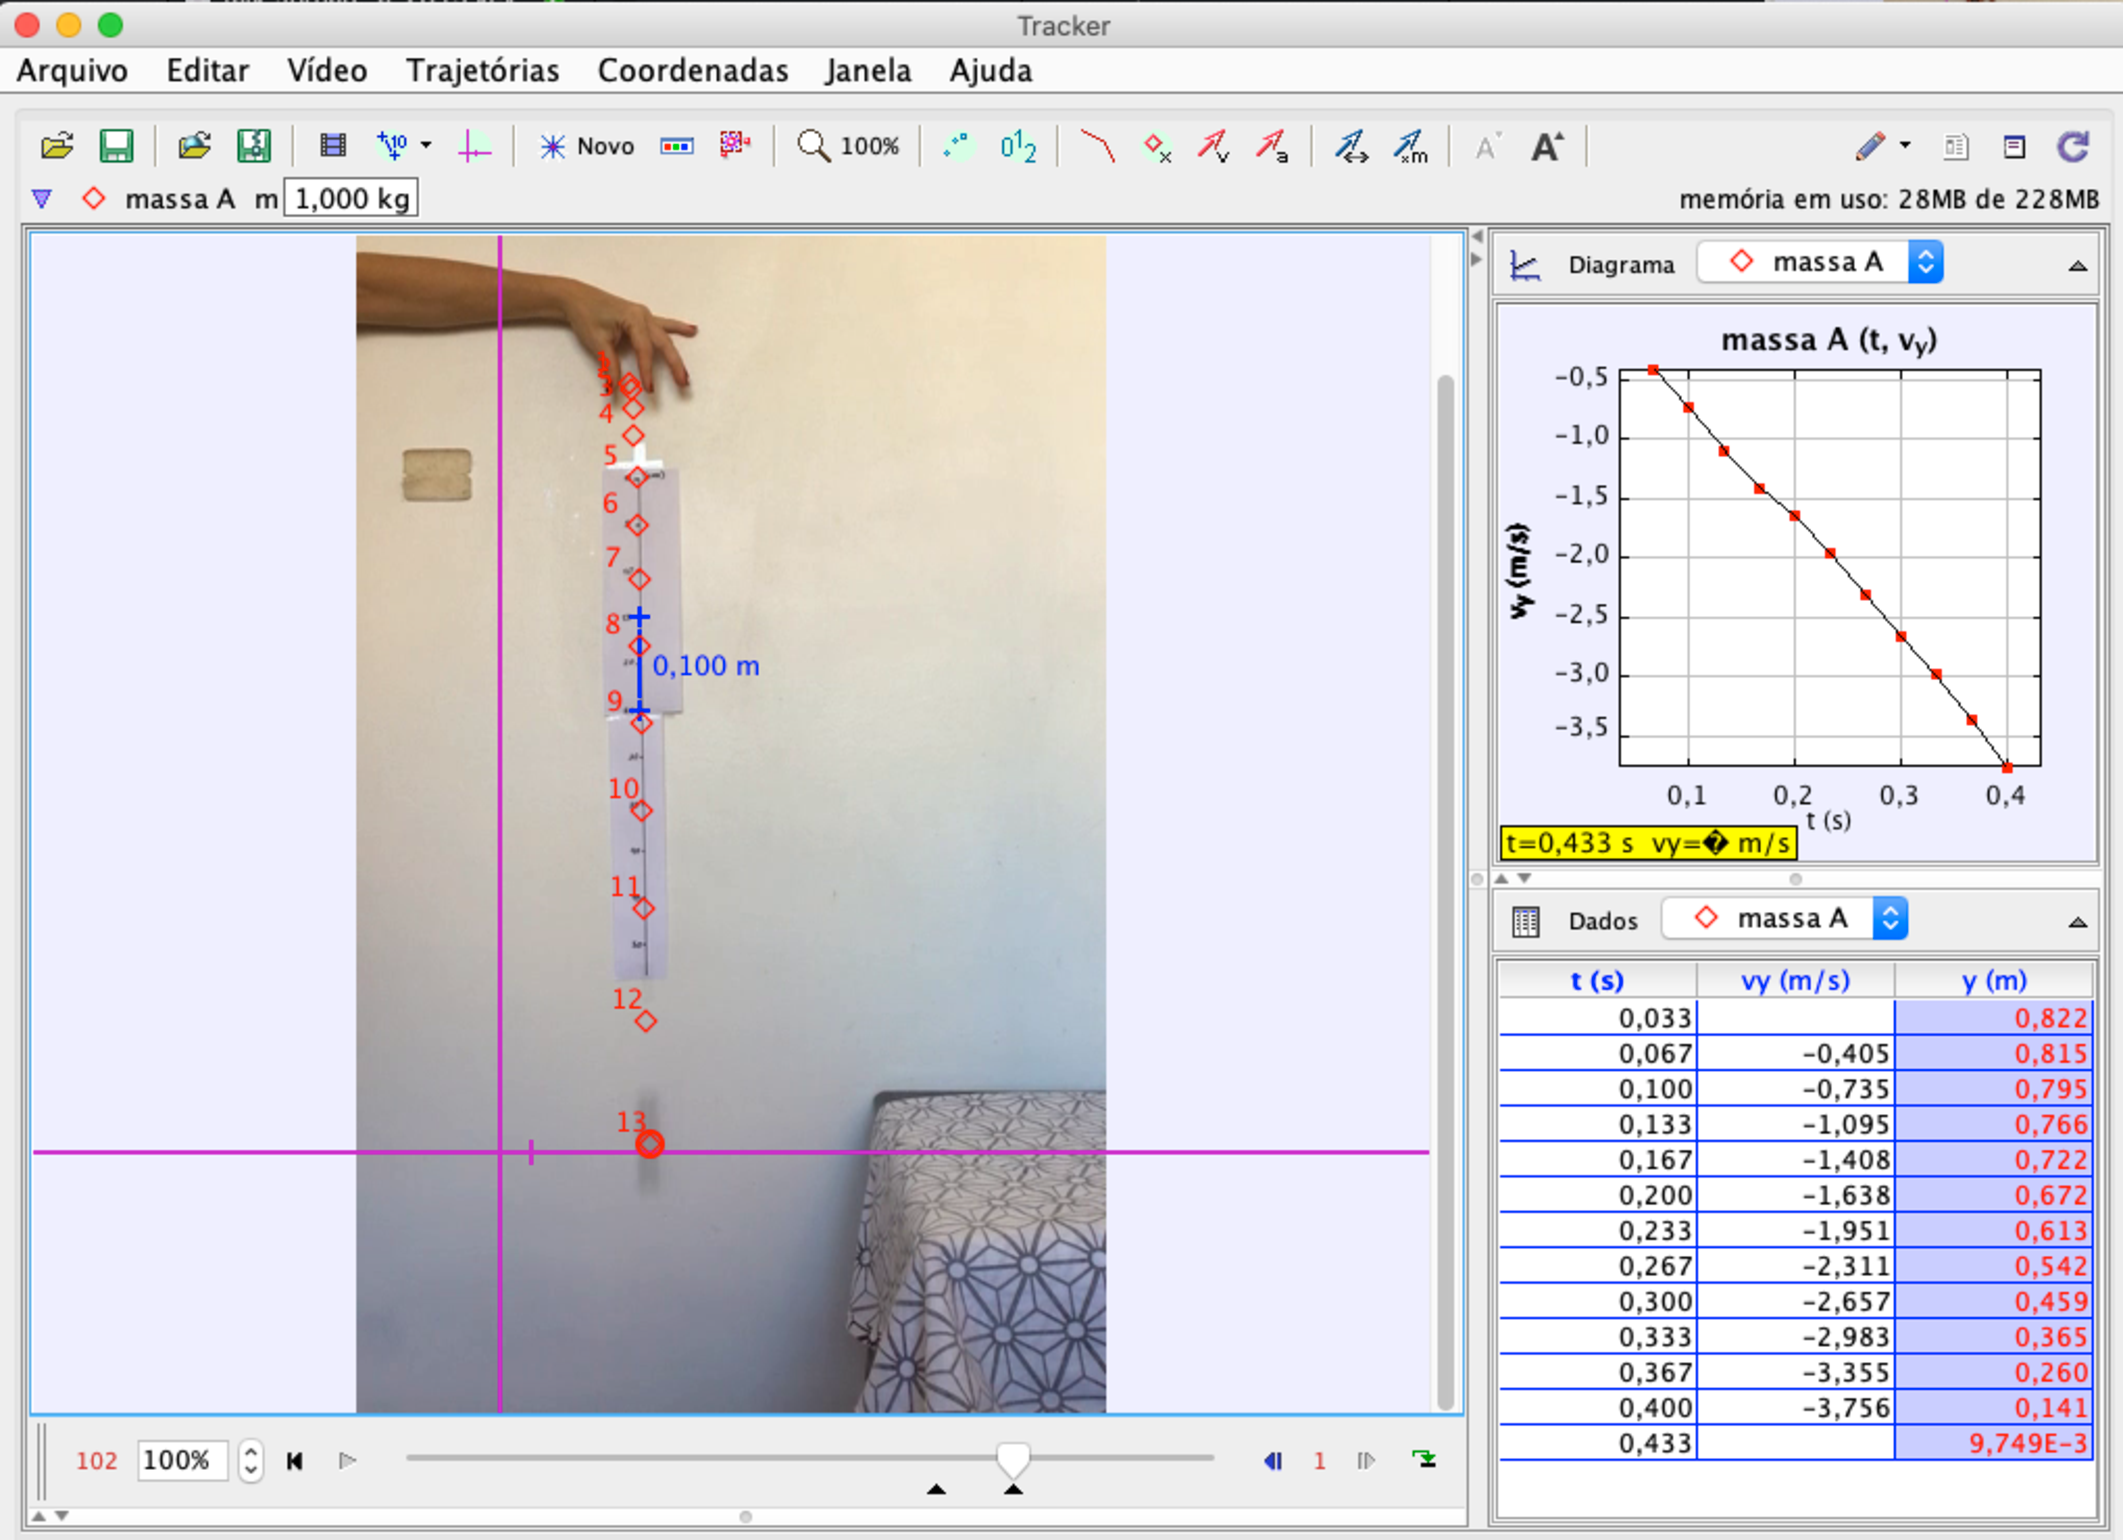
\includegraphics[width=9cm]{fig9AppB.pdf}
\caption{Pontos da trajetória marcados e dados coletados nas colunas da janela de tabela.}
\label{fig9AppB}
\end{figure}
No processo de medida é importante se auxiliar da ferramenta zoom, indicada pela seta laranja na 
Figura \ref{fig8AppB}, para ter uma melhor imagem da bolinha e poder determinar com melhor precisão o seu centro. Uma vez escolhido um zoom (por exemplo 400\%) para enquadrar a imagem 
da bolinha arraste a imagem com o mouse. Na Figura \ref{fig9AppB} é mostrado 
o final do processo de medida. Fazendo doble click, com o botão esquerdo do mouse, no cabeçalho de uma coluna, na janela de tabela, você seleciona a janela e os valores ficaram da cor rosa como estão os valores da coordenada ``y''na Figura \ref{fig9AppB}. Uma vez selecionada a 
coluna, fazendo click com o botão direito do mouse você abrira uma janela com varias opções.
Na aba ``Números'' você poderá escolher o formato (sem com vírgula ou ponto para separar os decimais). Uma vez escolhido o formato você poderá copiar os dados selecionados para serem transferidos, por exemplo, para uma planilha tipo Excel. 
 
\clearpage

%-----------------------------------------------------------------------------------------------------------------
\section{Apêndice C: Tutorial básico de uso do aplicativo VidAnalysis}
\label{ApendiceC}
 %-----------------------------------------------------------------------------------------------------------------
\indent
VidAnalysis é um aplicativo para análise física de movimentos em vídeos muito fáceis de usar.
O aplicativo é compatível com Android e pode ser baixado do Google Play gratuitamente em {\color{blue} https://play.google.com/store/apps/\\details?id=com.vidanalysis.free}, ou simplesmente pesquise no Google Play com o nome VidAnalysis free. O aplicativo possui apenas uma versão em inglês, mas devido à simplicidade de seu uso, ele não representa nenhum problema.

Para realizar a coleta de dados das posições do objeto gravado no vídeo, siga as etapas abaixo:

\underline{\bf Passo 1:} {\bf Abertura do vídeo a ser analisado}\\
\indent

Primeiro, temos que gravar um vídeo ou importar um existente. Se você decidir importar um vídeo, clique no sinal de adição mostrado com uma seta preta na Figura \ref{apendice1c}. Como o aplicativo VidAnalysis suporta apenas formatos de vídeo do tipo ``mp4'' é recomendável gravar  diretamente dentro do aplicativo, escolhendo a opção marcada pela seta vermelha na Figura \ref{apendice1c}.
\begin{figure}[h!]
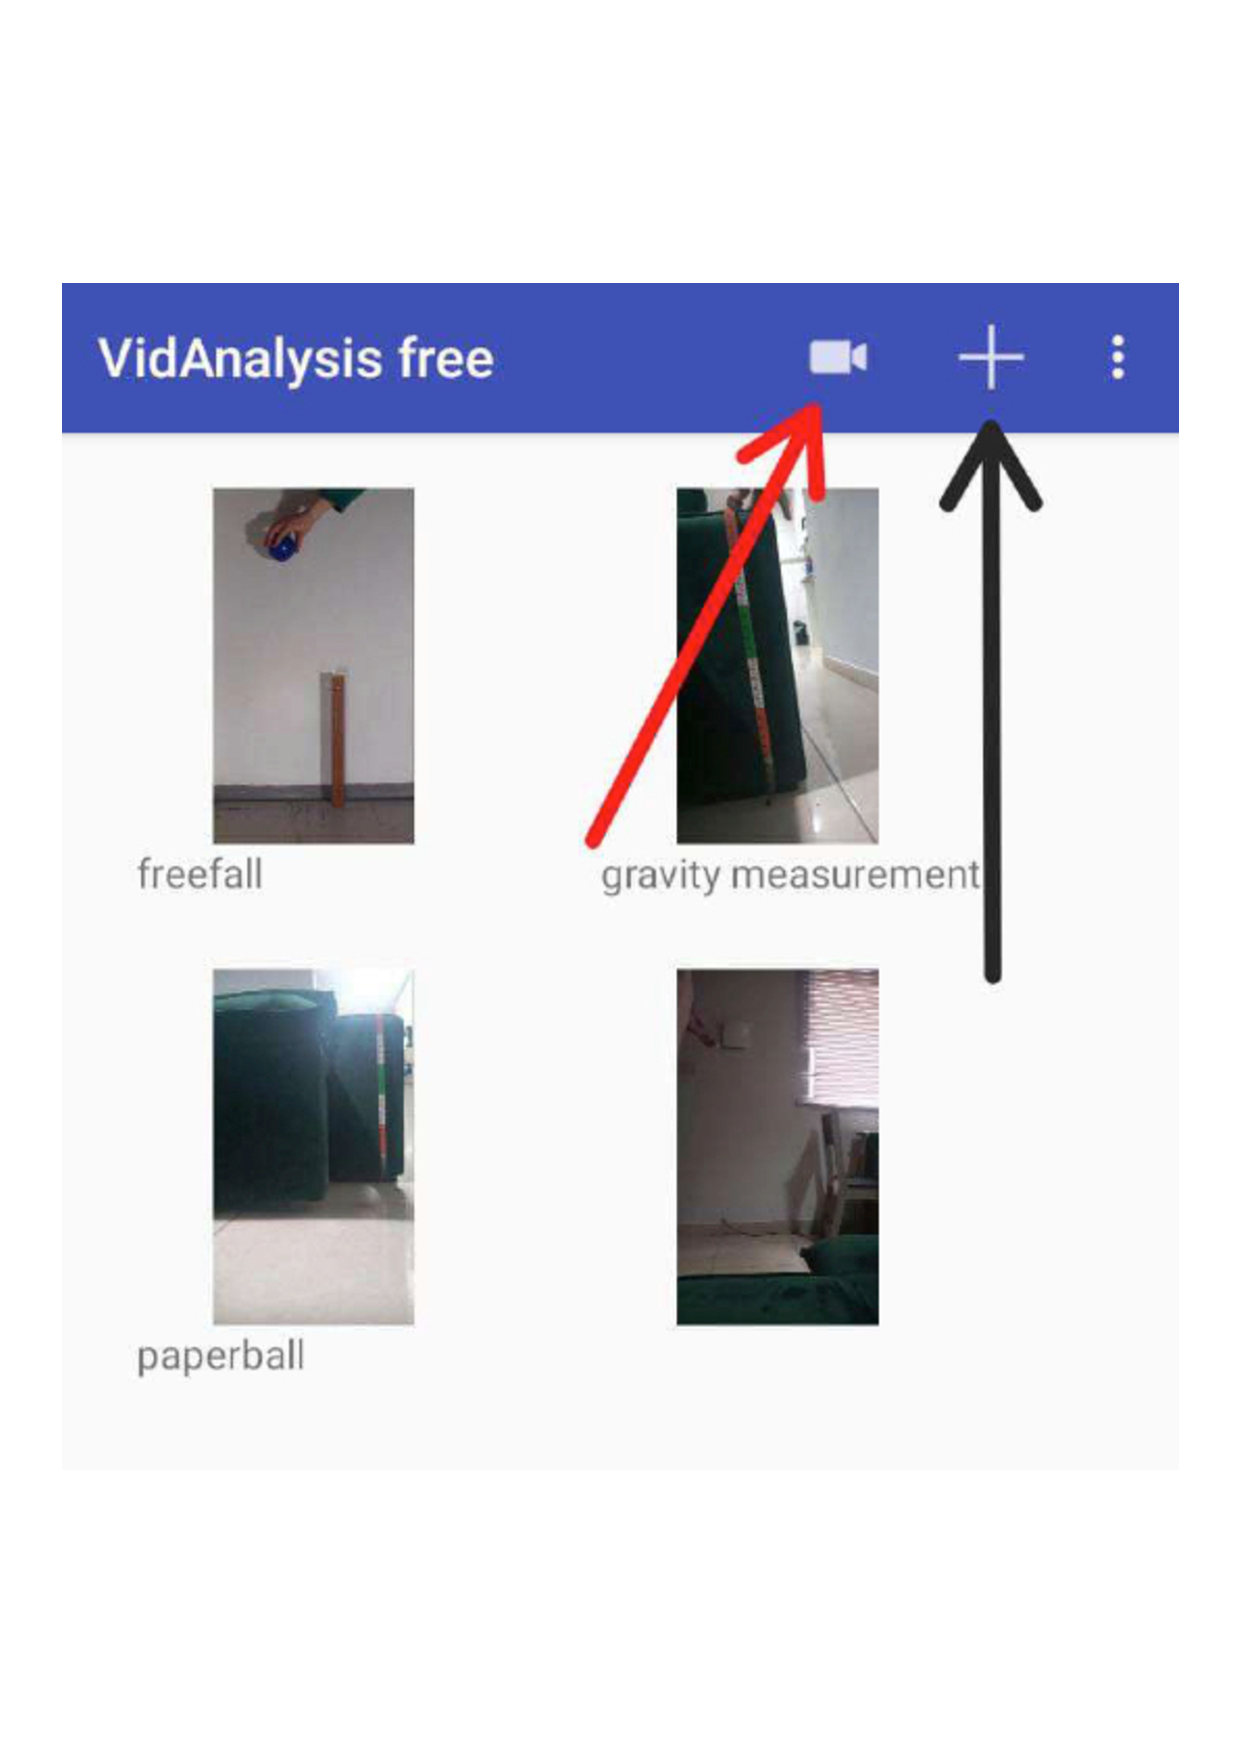
\includegraphics[width=9cm]{imagenapendicec1.pdf}
\caption{Menu do app VidAnalysis.}
\label{apendice1c}
\end{figure}
Ao capturar vídeos para análise, é importante que a câmera esteja fixa, que o movimento esteja dentro do plano da câmera, e que no vídeo gravado apareça alguma referencia de 
um comprimento conhecido, por exemplo de uma régua. 
\par
\vskip 0.5cm
\underline{\bf Passo 2:} {\bf calibração}\\
\indent

Para começar a análise do movimento do objeto primeiramente  
selecionamos o vídeo no reprodutor e será aberta a primeira imagem dele como se mostra na Figura \ref{apendice2c}. É importante avançar o vídeo nessa tela, para começar a coleta de dados da trajetória do objeto diretamente no momento em que o movimento  começa, para isso fazemos click no botão mostrado pela seta verde na Figura \ref{apendice2c} até avançarmos ao quadro do vídeo que interessa. Fazendo click nos três pontos indicado pela seta azul na Figura \ref{apendice2c}, conseguimos ocultar o menu em preto, para uma melhor visualização do vídeo.
\begin{figure}[h!]
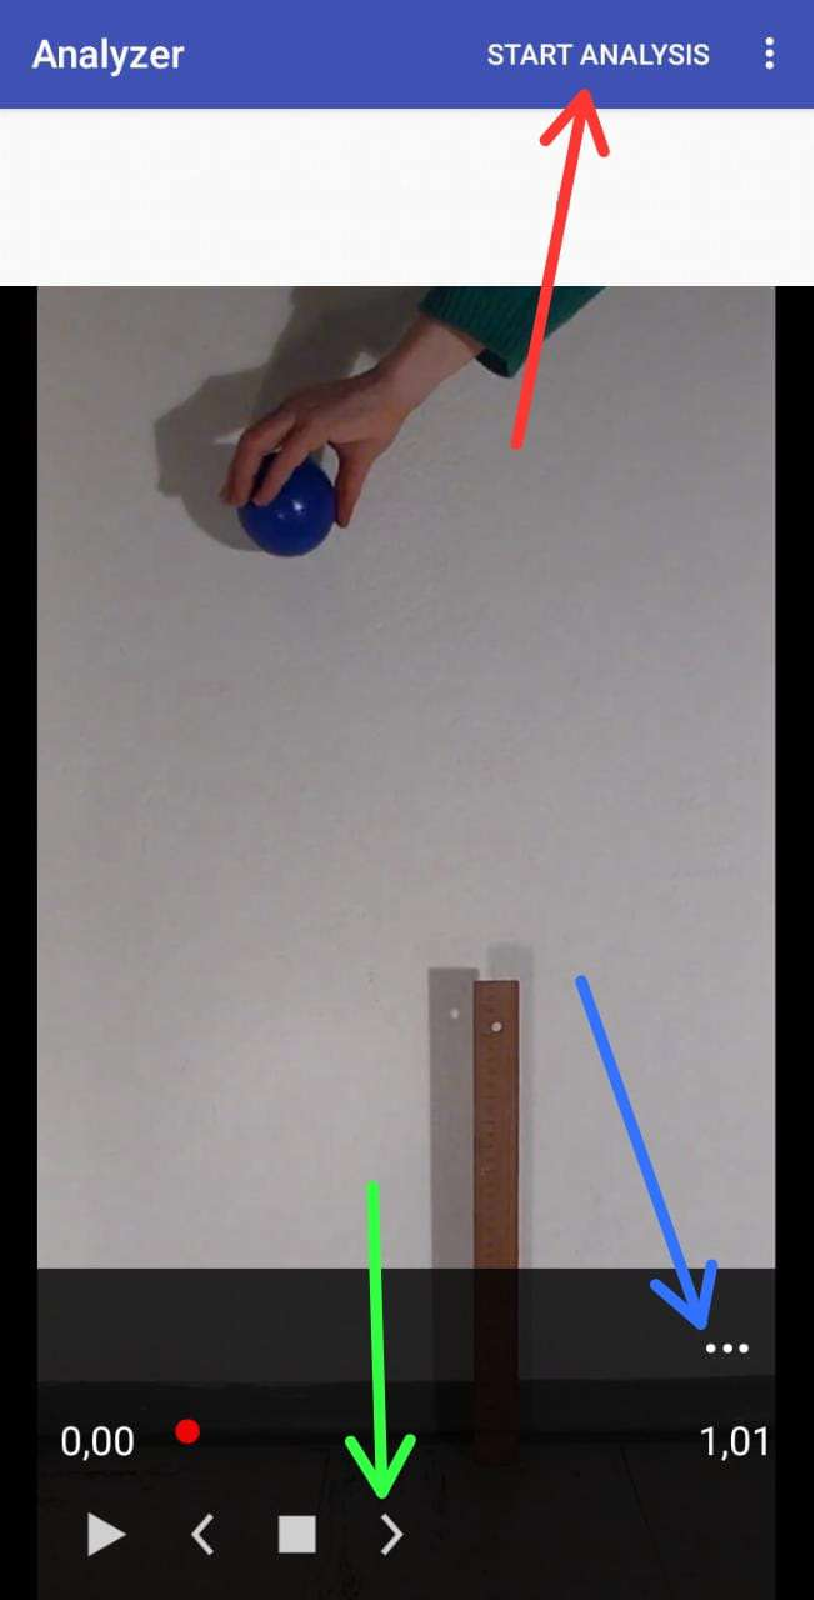
\includegraphics[width=9cm]{imagenapendicec2.pdf}
\caption{Reprodutor de video do aplicativo VidAnalysis.}
\label{apendice2c}
\end{figure}
Antes da coleta de dados deve primeiro calibrar qual é a escala de comprimentos que será usada pelo aplicativo. Para isso, fazemos click na aba ``start analysis''  no canto superior direito na Figura \ref{apendice2c}. Agora temos que marcar o comprimento conhecido.
 Ao fazer click no ponto inicial do comprimento conhecido, na tela esse ponto será marcado com uma cruz azul. Em seguida, deve fazer click novamente no ponto final do comprimento conhecido e outra cruz azul indicará esse ponto. Após finalizar essa segunda marcação abrirá imediatamente uma janela solicitando o tamanho conhecido, como mostramos na Figura \ref{apendice3c}. A legenda em inglês na janela pergunta ``Qual é o comprimento real disto em metros'' (``How many meters is this in real'' em inglês). É importante saber que a unidade a ser usada pelo aplicativo para comprimentos é sempre metros portanto as velocidades serão em metros por segundo por exemplo.
\begin{figure}[h!]
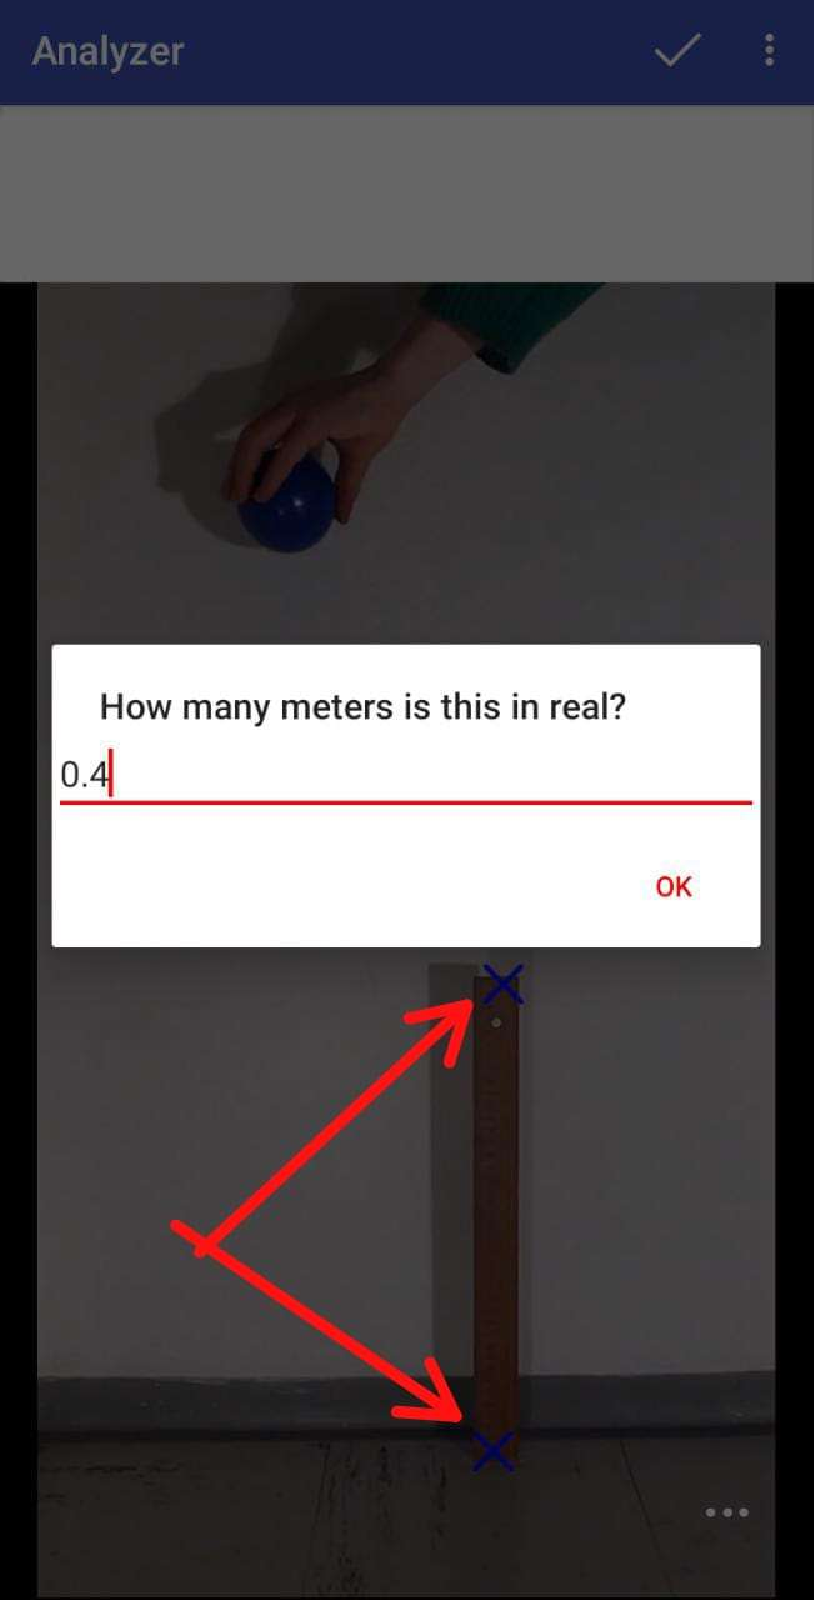
\includegraphics[width=9cm]{imagenapendicec3.pdf}
\caption{Escolha da escala de comprimentos no reprodutor de vídeo do aplicativo VidAnalysis, a ser usado na tomada de dados dos pontos da trajetória do objeto.}
\label{apendice3c}
\end{figure}
Após dar ``ok'' na janela da escala aparecerá um sistema de eixos coordenados cuja origem devemos estabelecer (ver Figura  \ref{apendice4c}). Em geral, é uma boa ideia posicionar a origem de coordenadas de tal maneira que as coordenadas da posição do objeto sempre tenham o mesmo sinal ao longo da trajetória.
\begin{figure}[h!]
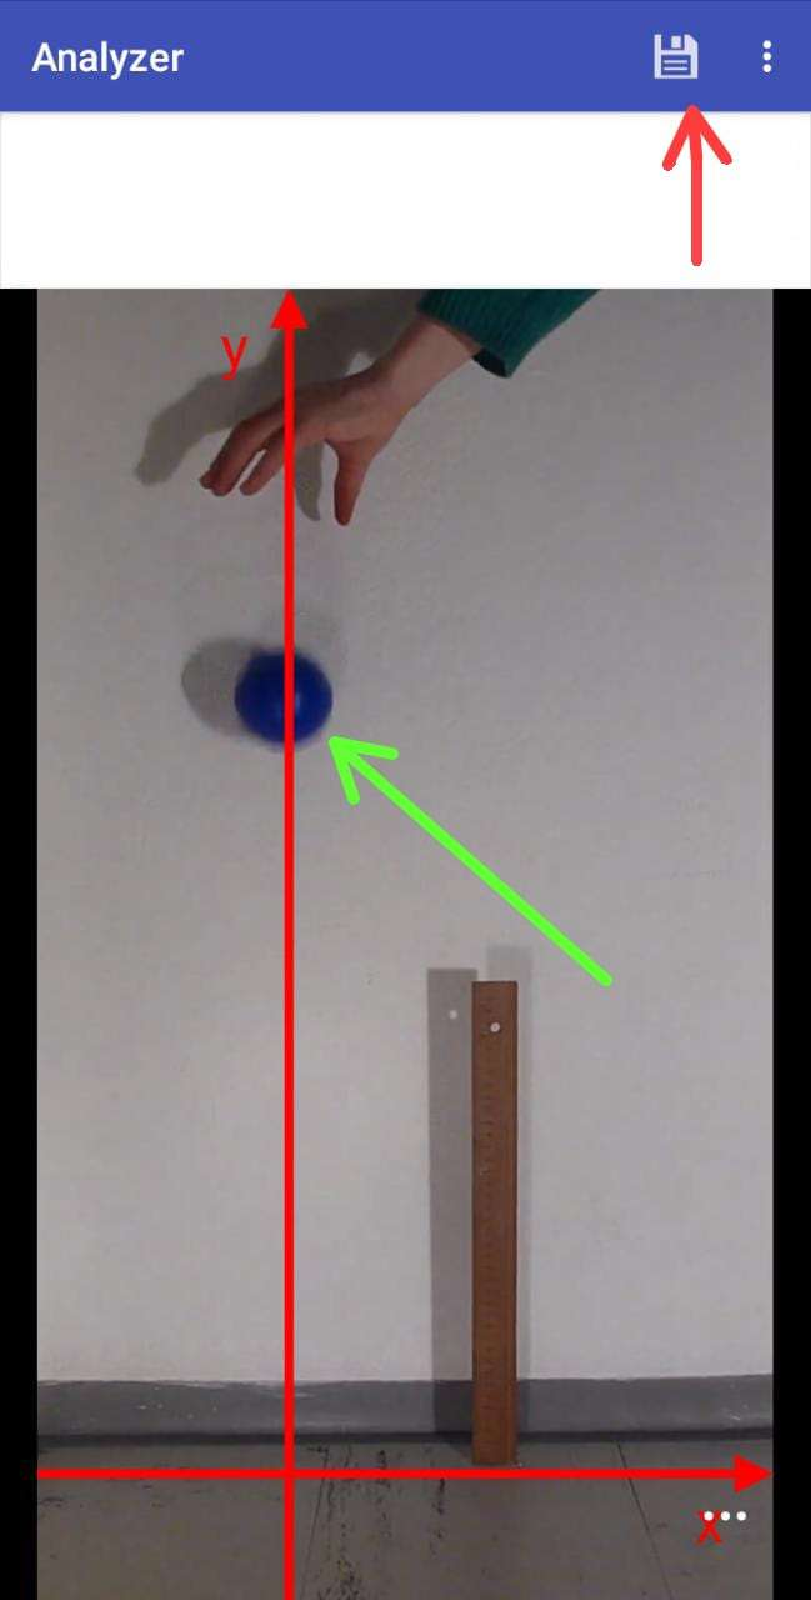
\includegraphics[width=9cm]{imagenapendicec4.pdf}
\caption{Sistema de eixos no reprodutor de vídeo do aplicativo VidAnalysis.}
\label{apendice4c}
\end{figure}
\par
\vskip 0.5 cm
\underline{\bf Passo 3:} {\bf coleta de dados}\\
\indent

A coleta de dados começa fazendo um click com o dedo no ponto do objeto que queremos seguir a trajetória, por exemplo no meio da bolinha azul na Figura \ref{apendice4c}. Como as marcações são feitas com o dedo sugerimos que o corpo, cuja trajetória será determinada, seja suficientemente grande.
Depois que o primeiro click for feito, uma cruz azul aparecerá e o vídeo avançará alguns quadros. O intervalo de tempo transcorrido, medido em segundos, entre um click e outro e automaticamente determinado pelo programa. Vamos fazer click novamente tantas vezes como seja necessário para acompanhar a evolução da posição do objeto entre a posição inicial e final previamente estabelecidas. Leve em conta que para uma bolinha em queda vertical uma distância percorrida de um metro é o mínimo necessário para efetuar a análise, mas também não é necessário acompanhar 
todo o movimento do corpo até o chão.
\par 
Como mostrado na Figura \ref{fig2},  pode ser que ao longo da trajetória não vejamos o corpo em questão claramente definido em uma única posição, mas como uma imagem embaçada devido à alta velocidade do mesmo. Então para determinar a posição do centro da bolinha e a sua incerteza siga as orientações indicadas nessa figura e no texto ao lado dela. 
\par
\vskip 0.5cm
\underline{\bf Passo 4:} {\bf salvar dados}\\
\indent

Depois de determinados todos os pontos da trajetória do corpo, basta pressionar o botão ``Salvar', conforme mostrado pela seta vermelha na Figura \ref{apendice4c}. Após o click se abrirá uma janela 
com a frase ``Nome para a análise'' (``Name for analysis'' em inglês). Uma vez escrito o nome do arquivo de dados dê click em ``ok'' e imediatamente verá uma janela na qual você poderá navegar. 
Rolando a imagem, no final aparecerá uma tabela com várias colunas de dados como mostrada na Figura \ref{apendice5c}.
É possível também exportar essa tabela de dados  para um arquivo que é uma planilha no formato ``.cvs'' (``comma separated values'''), que poderá ser lida por um programa de computador do tipo Excel. Mas também você poderá simplesmente copiar os dados que precisará (por exemplo 
a posição ``$y$'' como funçao do tempo ``$t$') numa folha de papel para continuar a análise. 
\par
Note que uma vez escolhido o nome do arquivo para a tabela de dados, esta tabela é automaticamente guardada pelo aplicativo. 
Para cada vídeo guardado dentro do aplicativo é possível realizar 
diferentes análises de dados e guardar cada um deles, dentro do aplicativo, 
com nomes diferentes.
Assim, por exemplo, na Figura \ref{apendice1c} vemos vários vídeos guardados.
Se algum desses vídeos já foi analisado, quando fizer click nele aparecerá uma janela com 
várias opções de escolha. A primeira diz ``Começar análises'' (``Start analysis'' em inglês), o que permitirá realizar uma nova tomada de dados. Embaixo aparecem as outras opções que são
os nomes dos diferentes arquivos de dados já guardados. Fazendo click num deles é possível visualizar seu conteúdo novamente. Note que desta maneira é possível guardar a trajetória de mais de uma massa cujo movimento estiver gravado no vídeo. Assim, por exemplo, no caso em que a colisão de dois ou mais corpos estiver gravada no vídeo, é possível guardar os dados da trajetória de cada um deles.  
\begin{figure}[h!]
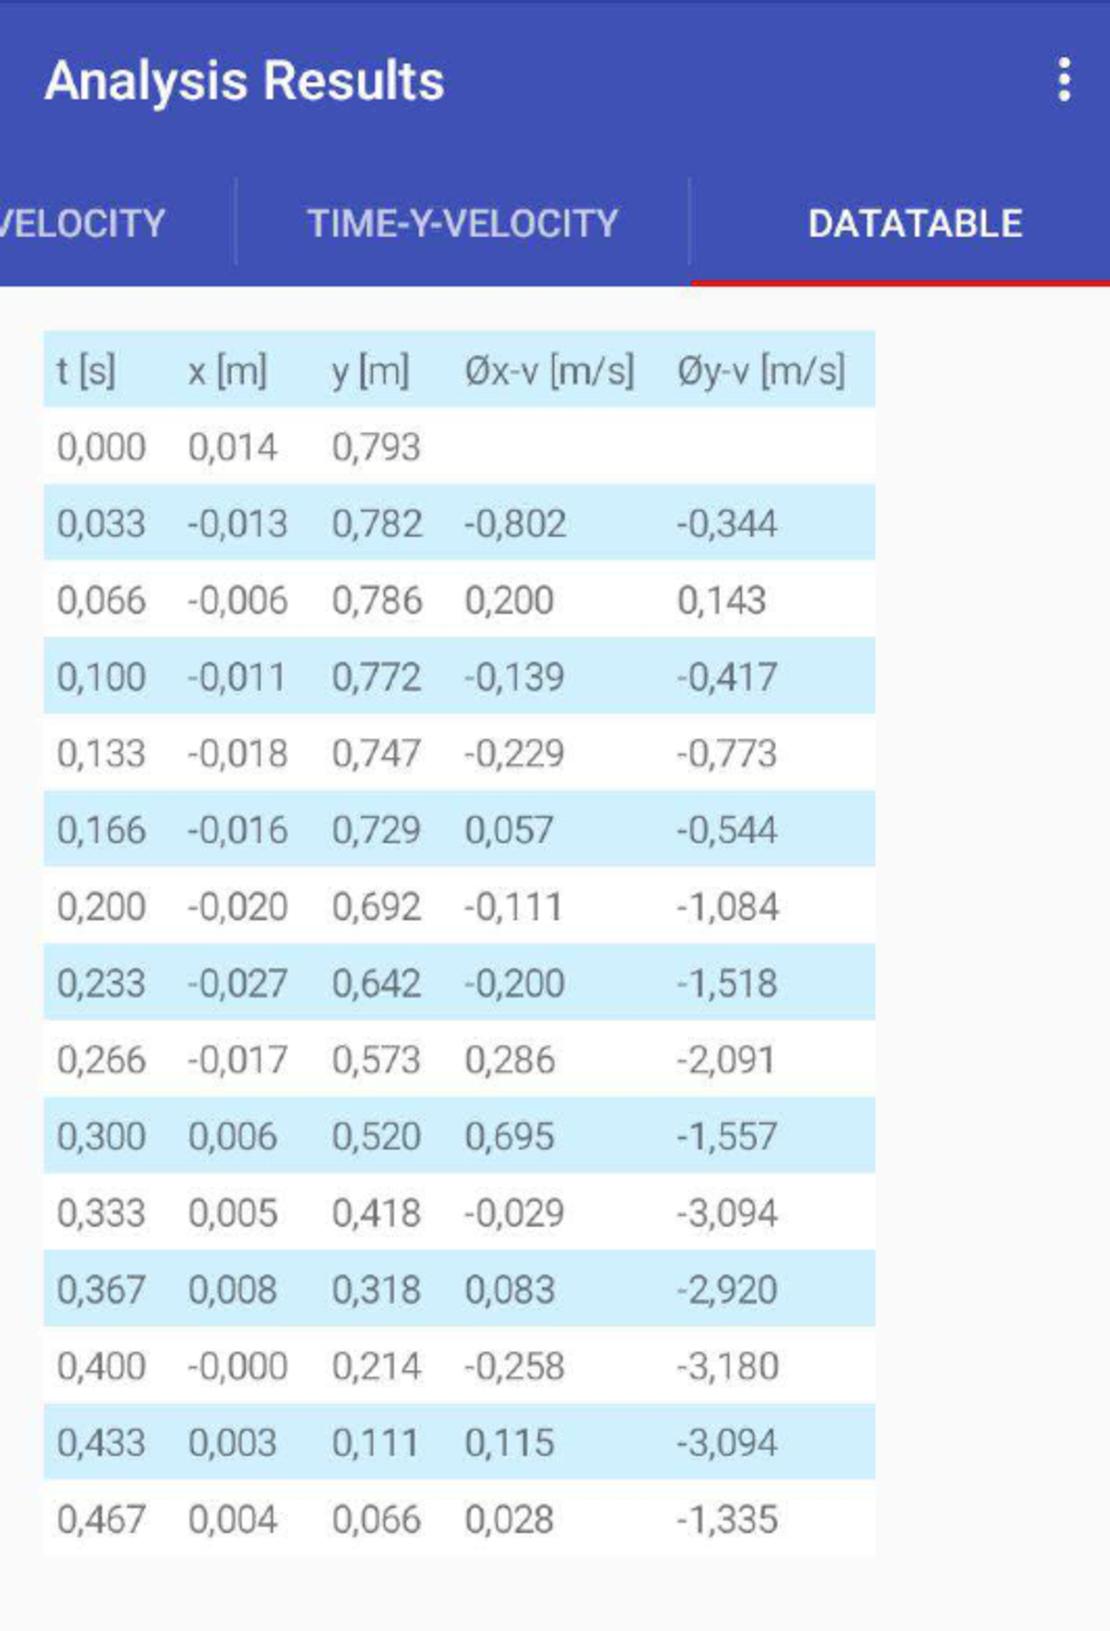
\includegraphics[width=9cm]{imagenapendicec5.pdf}
\caption{Tabela de dados gerada dentro do aplicativo VidAnalysis.}
\label{apendice5c}
\end{figure}
 \clearpage
 %-----------------------------------------------------------------------------------------------------------------
\section{Apêndice D: Cálculo da velocidade num MRUV.}
\label{ApendiceD}
 %-----------------------------------------------------------------------------------------------------------------
\indent 

No movimento uniformemente acelerado a velocidade da partícula em um instante t pode ser calculada a partir da velocidade média calculada entre os instantes $t+\Delta t$ e $t-\Delta t$ 
com $\Delta t$ constante. Isto é:
\beq
\langle v_y(t) \rangle=\frac{y(t+\Delta t)-y(t-\Delta t)}{2\Delta t}.
\eeq
Assim, para um conjunto de medições de posição em função do tempo, podemos calcular a velocidade em cada ponto $(i)$ a partir das medições de tempo e posição do ponto posterior
$(t_{i+1}$ e $y_{i+1})$ e anterior $(t_{i-1}$ e $y_{i-1})$, utilizando a fórmula:
\beq
v_{y,i}=\frac{y_{i+1}-y_{i-1}}{t_{i+1}-t_{i-1}}.
\eeq
Para cada valor de velocidade também podemos calcular a incerteza associada mediante a fórmula de propagação de incertezas. Desprezando a incerteza na determinação do tempo, obtemos:
\beq
\delta_{v_{y,i}}=\frac{\delta^2_{y_{i+1}}+\delta^2_{y_{i-1}}}{(t_{i+1}-t_{i-1})},
\eeq
com $\delta^2_{y_{i+1}}$ e $\delta^2_{y_{i-1}}$ as incertezas na determinação da posição $y_{i+1}$
e $y_{i-1}$ respectivamente.

\clearpage

 %-----------------------------------------------------------------------------------------------------------------
\section{Apêndice E: Método gráfico para ajustar uma reta com incerteza.}
\label{ApendiceG}
 %-----------------------------------------------------------------------------------------------------------------
\indent 

Se medimos duas variáveis, $X$ e $Y$, cuja relação sabemos que é linear, podemos encontrar uma relação analítica que melhor ajuste nossos dados. No Capítulo 4 da parte Conceitos Básicos na apostila discutimos como isto é feito analiticamente mediante o método de mínimos quadrados, mas aqui estudaremos como faze-lo a partir do gráfico de $Y$ em função de $X$, o que chamamos de 
método gráfico.
Na figura seguinte podemos observar a distribuição dos dados, círculos abertos, que queremos ajustar. Neste caso, para simplificar, vamos considerar que a incerteza associada a cada medida é do tamanho do ponto. Para ajustar graficamente os pontos por uma reta que melhor representa a 
variação de $Y$ em função de $X$ devemos traçar uma reta de forma tal que os pontos que se situem ``acima'' da reta se vejam compensados pelos pontos que se situem ``abaixo'' da mesma, como na linha cheia mostrada na Figura \ref{fig1AppG} \footnote{Note que o uso de uma régua transparente é conveniente pois permite ter uma visão global de todos os pontos.}.
\begin{figure}[h!]
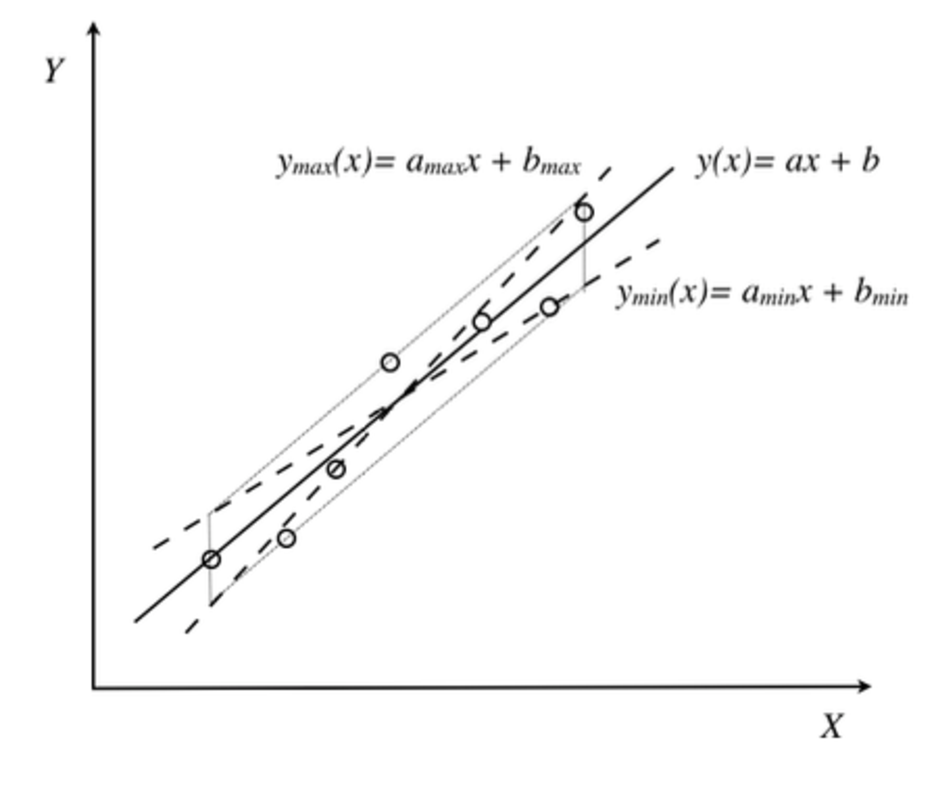
\includegraphics[width=9cm]{fig1AppG.pdf}
\caption{Os círculos representam os pontos experimentais e a linha cheia é
o melhor ajuste linear a esses dados. }
\label{fig1AppG}
\end{figure}
Desta forma podemos determinar o coeficiente angular $(a)$ e linear $(b)$ para a equação da reta 
$y=ax+b$. Mas mesmo no caso gráfico é preciso dar as incertezas associadas à determinação de 
$a$ e $b$. Para isto, vamos traçar duas linhas paralelas à melhor reta $(R)$ que ajusta os nossos dados encontrados, uma passando pelo ponto mais afastado ``acima'' da reta $R$ e outra pelo ponto mas afastado ``abaixo'' da reta $R$. Caso exista um outro ponto excepcionalmente afastado da reta média poderá não ser considerado pois a probabilidade de corresponder a uma medida incorreta é grande. Obtendo a interseção destas
retas por duas retas paralelas ao eixo-$y$ que contêm o primeiro e último ponto experimental representado temos um ``paralelogramo de incerteza'' como é mostrado na Figura
\ref{fig1AppG} (paralelogramo pontilhado). A partir deste, desenhamos as duas retas diagonais achando o que chamaremos a reta de máxima $y_{max}=a_{max}x+b_{max}$ e a de mínima 
$y_{min}=a_{min}x+b_{min}$ (ver Figura \ref{fig1AppG}).
\par
A partir destas três retas, podemos então determinar as incertezas associadas para o 
coeficiente angular $\delta a$ e linear $\delta b$ como:
\bse
\bea
\delta a&=&\frac{a_{max}-a_{min}}{2}\\
\delta b&=&\frac{b_{max}-b_{min}}{2}
\eea
\ese


\end{document}
